\documentclass[12p]{article}

\usepackage{geometry} % Required to change the page size to A4
\geometry{a4paper} % Set the page size to be A4 as opposed to the default US Letter

\usepackage[utf8]{inputenc}
\usepackage{graphicx}
\usepackage{float} % Allows putting an [H] in \begin{figure} to specify the exact location of the figure
\usepackage{wrapfig} % Allows in-line images such as the example fish picture
\usepackage[nopar]{lipsum} % Used for inserting dummy 'Lorem ipsum' text into the template
\usepackage{fancyhdr}
\usepackage[parfill]{parskip} % Makes sure to put line breaks in between paragraphs and have no indentation
\usepackage{dirtytalk} % Used for quotations (\say{quote})
\usepackage[toc,page]{appendix}
\usepackage{caption}
\usepackage{subcaption}
\usepackage{url}
\usepackage{minted} % Used for including code with syntax highlighting: https://www.sharelatex.com/learn/Code_Highlighting_with_minted
\usepackage{fontawesome} % Allows usage of icons within text
\usepackage{enumitem}

\usepackage[
  style=numeric,
  sorting=none
  ]{biblatex}
\addbibresource{references.bib}

\linespread{1.2} % Line spacing
\setlength\parindent{0pt} % Globally suppress indentation
 
\graphicspath{{pics/}} % Specifies the directory where pictures are stored

\pagestyle{fancy} % Use this, if a header on each page with the section title and page number is wanted
\fancyhf{} % Removes all headers and footers, comment this to show page number at the bottom of each page again
\fancyhead[L]{\rightmark} % Sets the section title on the left side of the header
\fancyhead[R]{\thepage} % Sets the page number on the right side of the header

\newcommand{\HRule}{\rule{\linewidth}{0.5mm}} % Defines a new command for horizontal lines
\newcommand{\SlimHRule}{\rule{\linewidth}{0.25mm}} % Defines a new command for horizontal lines

%----------------------------------------------------------------------------------------

\begin{document}

%----------------------------------------------------------------------------------------
%	TITLE PAGE
%----------------------------------------------------------------------------------------

\begin{titlepage}
  
  \center
  
  %------------------------------------------------
	%	Logo
	%------------------------------------------------
	
	
\includegraphics[width=0.2\textwidth]{pics/AAU_Logo.png}\\[1cm]
  
  %------------------------------------------------
	%	Headings
	%------------------------------------------------
	
	\textsc{\LARGE Aalborg University Copenhagen}\\[1.5cm]
	
	\textsc{\Large P1 Project}\\[0.5cm]
	
	\textsc{\large Group 007}\\[0.5cm]
	
	\textsc{\large IT, Communication and New Media}\\[0.5cm]
	
	
	%------------------------------------------------
	%	Title
	%------------------------------------------------
	
	\HRule\\[0.4cm]
	
	{\huge\bfseries Gangster Squirrel}\\[0.4cm]

	\HRule\\[1.5cm]
	
	%------------------------------------------------
	%	Author(s) and Supervisor(s)
	%------------------------------------------------
	
	\begin{minipage}{0.4\textwidth}
  \begin{flushleft} \large
  \emph{Authors}\\
    Ludvig Alexander \textsc{Brüchmann} \\
    Muheb \textsc{Khan} \\
  	Rehan \textsc{Mir} \\
  	Johannes \textsc{Mols} \\
  	Martin \textsc{Sander} \\
  	Agata \textsc{Surmacz} \\
  	Boris \textsc{Yordanov} \\
  \end{flushleft}
  \end{minipage}
  ~
  \begin{minipage}{0.4\textwidth}
  \begin{flushright} \large
  \emph{Study Numbers} \\
    20174692 \\
    20173803 \\
    20174693 \\
    20174921 \\
    20174446 \\
    20173800 \\
    20174447 \\
  \end{flushright}
  \end{minipage}\\[0.5cm]
  
  %------------------------------------------------
  
  \begin{minipage}{0.4\textwidth}
  \begin{flushleft} \large
  \emph{Supervisor}\\
    Morten \textsc{Falch} \\
  \end{flushleft}
  \end{minipage}
  ~
  \begin{minipage}{0.4\textwidth}
  \begin{flushright} \large
  \end{flushright}
  \end{minipage}\\[0.5cm]

	%------------------------------------------------
	%	Date
	%------------------------------------------------
	
	\vfill\vfill\vfill % Position the date 3/4 down the remaining page
	
	{\large\today} % Date, change the \today to a set date if you want to be precise
	
  
\end{titlepage}

%----------------------------------------------------------------------------------------
%	SYNOPSIS / ABSTRACT
%----------------------------------------------------------------------------------------

\begin{abstract}
\thispagestyle{plain} %Sets the page style for this specific page to plain, to remove the header and show the page number at the bottom
  This is our Abstract, my dudes.

\end{abstract}

\newpage

%----------------------------------------------------------------------------------------
%	TABLE OF CONTENTS
%----------------------------------------------------------------------------------------

\tableofcontents % Include a table of contents
\thispagestyle{plain} %Sets the page style for this specific page to plain, to remove the header and show the page number at the bottom

\newpage % Begins the essay on a new page instead of on the same page as the table of contents 

%----------------------------------------------------------------------------------------
%	INTRODUCTION
%----------------------------------------------------------------------------------------

\section{Problem Introduction} \label{ProblemIntroduction}

Video games have formed a niche in pop culture comparable to the film or music industry. Although the latter have many sources of revenue - direct sales, rental licenses, sales via broadcasting networks etc, video games have essentially one source - selling directly to it’s customers. Despite that the gaming industry has surpassed the music industry in revenue, reaching \$64.9 billion (globally) in 2014, compared to the film industry’s \$90 billion and \$20.97 for the music sector.\cite{UnderstandingVideoGames}

A video game has high production costs (similar to a film or music album), which causes the market to be dominated by a few large companies, who can afford the costs of building a game. 90\% of revenue is generated by 10\% of the games.\cite{UnderstandingVideoGames}

The rising cost of game development is contributed by their increasing complexity. Even though there are successful games without storylines - think Tetris, a puzzle game, released in the mid 1980’s, which still remains popular amongst many age groups. On the other hand, most modern games, especially role playing games (RPGs) rely heavily – almost entirely - on a captivating story. In reality, an RPG is mostly like a movie for some players—where the actual gameplay easily becomes an addition to the intriguing story.\cite{GameDevelopmentEssentials}

\section{Problem formulation} \label{ProblemFormulation}

How can game developers attract interest in today’s saturated market? Retro games didn’t need anything else except an interesting gameplay. Modern game need an enticing storyline to make it.

\section{Project Delimitations} \label{ProjectDelimitations}

Our team decided to focus on building a working MVP for PC only, with only the most important features of the game - at least two levels, different enemies and weapons and statistics tracking. Given more time we would implement the missing parts of the game we had planned - more levels, ranged weapons, a navigational menu, a mobile version and implementing a marketing strategy, however for this project we decided that is out of scope.

\section{Project Introduction} \label{ProjectIntroduction}

Coming up with a story with the range and depth of a book or film, like popular game titles. We decided to make our game entertaining by making it comedic and including more pop culture references. We decided on this approach after learning of the success of games like Goat Simulator \cite{GoatSimulator} or I Am Bread \cite{IAmBread}.

Our game revolves around 24 hours of an action packed day of our main character - the Gangster Squirrel. He is a white-tailed antelope ground squirrel, which is the only squirrel who exhibits carnivorous behaviour \cite{CarnivorousSquirells} and therefore the most "gangsta". However, because it is a ground squirrel it’s not good at climbing trees so it needs items to help it climb.
Goal: it needs to get to the top of the tree to steal the eggs of the eagle - Pablo Escobar, which are full of pure columbian cocaine. It needs the drugs so it can sell it and pay the bail for it’s best friend - the Rasta Lion (sacred in Rastafarian culture \cite{RastaLion}). Rasta Lion is in jail for shooting the sheriff \cite{Sheriff} of the jungle.

To help achieve his goal, the player has access to the follwing items.

Equipment:
\begin{itemize}
  \item A backpack that holds all it’s items, that can be upgraded 
  \item Climbing boots
  \item Climbing kits which increase speed
  \item Climbing hat that adds armour
\end{itemize}

Melee Weapons:
\begin{itemize}
  \item Tree branch 
  \item Swiss army knife
  \item Switchblade
  \item Katana
\end{itemize}

Ranged Weapons:
\begin{itemize}
  \item Nuts
  \item Rocks
  \item Slingshot
  \item Machine gun
  \item Grenade Launcher
\end{itemize}

But he has to a lot of obstacles to overcome.

Enemies:
\begin{itemize}
  \item Frogs
  \item Birds
  \item Monkeys
\end{itemize}

Levels:
\begin{itemize}
  \item Ground - you need to defeat the enemies from the base of the tree so you can start climbing
  \item Tree - you need to defeat the enemies in the tree as you make your way to the last level
  \item Nest - you are in the nest and you need to defeat the eagle. If you beat it you get to choose if you take all it’s eggs or just the amount you need with rewards/punishments for each choice. Example: if you take all the coke you are busted by the police when you are climbing down the tree and tried as a dealer not user.
\end{itemize}


%----------------------------------------------------------------------------------------
%	METHODOLOGY
%----------------------------------------------------------------------------------------

\newpage
\section{Methodology} \label{Methodology}

%----------------------------------------------------------------------------------------
%	STATE OF THE ART
%----------------------------------------------------------------------------------------

\newpage
\section{State of the art}

In this section we have been looking for inspirations for our project. We have identified many of other games that are congruous to what we wanted to do.
We were looking for our competitors via Google and we also knew a few of them beforehand. We have found plenty of examples on the Internet and we chose the ones that are, in our opinion, the most similar and related to our game idea. Through this research we wanted to get an overview of general features that this type of games have. Then we decided to discuss which of them were the most relevant and which we would like to implement. This section also helped us to understand the market that we are working in and decide what our pricing and platform support we should offer.

%------------------------------------------------

\subsection{Tallowmere} \label{StateOfTheArt_Tallowmere}

\begin{figure}[ht]
  \center
  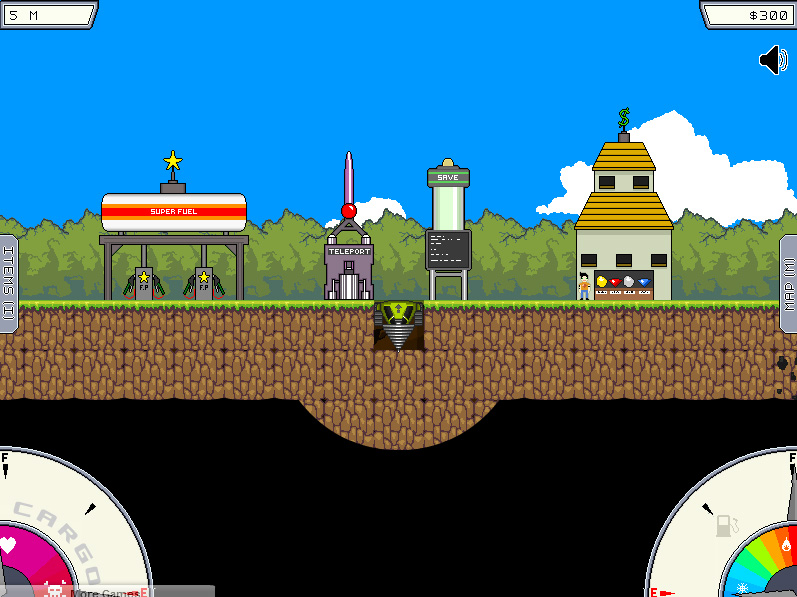
\includegraphics[width=0.8\textwidth]{StateOfTheArtScreenshots/mega_miner}
  \label{StateOfTheArt_Screenshots_Tallowmere}
  \caption{Screenshot of the game Mega Miner \cite{MegaMinerScreenshot}}
\end{figure}

A 2D action platformer with an emphasis on executing your hero's jumping, shield-blocking, and weapon-attacking at the right moments as you move through a procedurally-generated dungeon. The game is available for:

\emph{Windows XP SP2 or newer, macOS 10.8 or newer, SteamOS, Ubuntu 12.04, Android 4.4 or newer, iOS 8.1 or newer, Wii U}

Features:

\begin{itemize}
  \item Randomly-generated rooms, with each room bigger than the last
  \item Blood splats, particle effects and sounds
  \item Skill-based gameplay, with no ammo, mana, or stamina gauges
  \item Traps and obstacles to dodge and avoid
  \item Special boss and event rooms
  \item Different weapons, shields and garments the hero can equip
  \item Infinite jumping
  \item Single Player and local co-op (up to 4 players)
  \item Permanent death, with a typical run lasting from 1 minute to 2 hours depending on skill
\end{itemize}

Prices:

\begin{itemize}
  \item Steam: 3.99 EUR
  \item iTunes: 1.99 USD
  \item PlayStore: 16.0 DKK
\end{itemize}

%------------------------------------------------

\subsection{Cave Story Plus}

\begin{figure}[ht]
  \center
  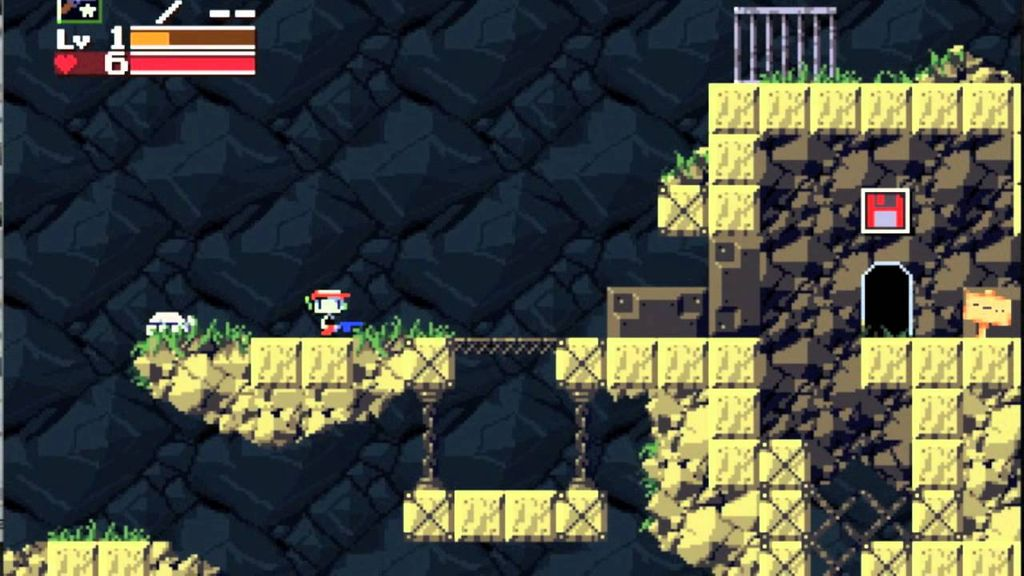
\includegraphics[width=1\textwidth]{StateOfTheArtScreenshots/cave_story_plus}
  \label{StateOfTheArt_Screenshots_CaveStoryPlus}
  \caption{Screenshot of the game Cave Story+ \cite{CaveStoryPlusScreenshot}}
\end{figure}

Cave Story+ is a Cave Story remake for PC, Mac and Nintendo Switch developed by Nicalis. It was released on Steam on November 22, 2011. The game features remastered graphics and music as well as several new game modes, of which one is only made exclusively to the Nintendo Switch version \cite{CaveStoryPlusWiki}.

Cave story+ has a selection of three difficulty levels; easy, standard and hard. Easy mode halves the HP of enemies and halves the damage they do to Quote (the main protagonist of Cave Story). The standard difficulty, is identical to the original game, in which Quote takes 100\% damage, and enemies have 100\% HP. Hard mode doubles the HP of enemies and removes all Life Capsules but one from the game, leaving the player with a maximum of 8 HP. Moreover, the Missile Launcher isn't available in the Hard mode.

Features:

\begin{itemize}
  \item Background music
  \item Over 20 boss battle games
  \item A variety of weaponry
  \item Four different game endings
  \item Hard mode for veterans
  \item Multiple versions available
  \item Metroid inspired setting
  \item Simple storyline
\end{itemize}

Prices:

\begin{itemize}
  \item Steam: 14.99 EUR
  \item iTunes: 4.99 USD
\end{itemize}

%------------------------------------------------

\subsection{Stardew Valley}

\begin{figure}[ht]
  \center
  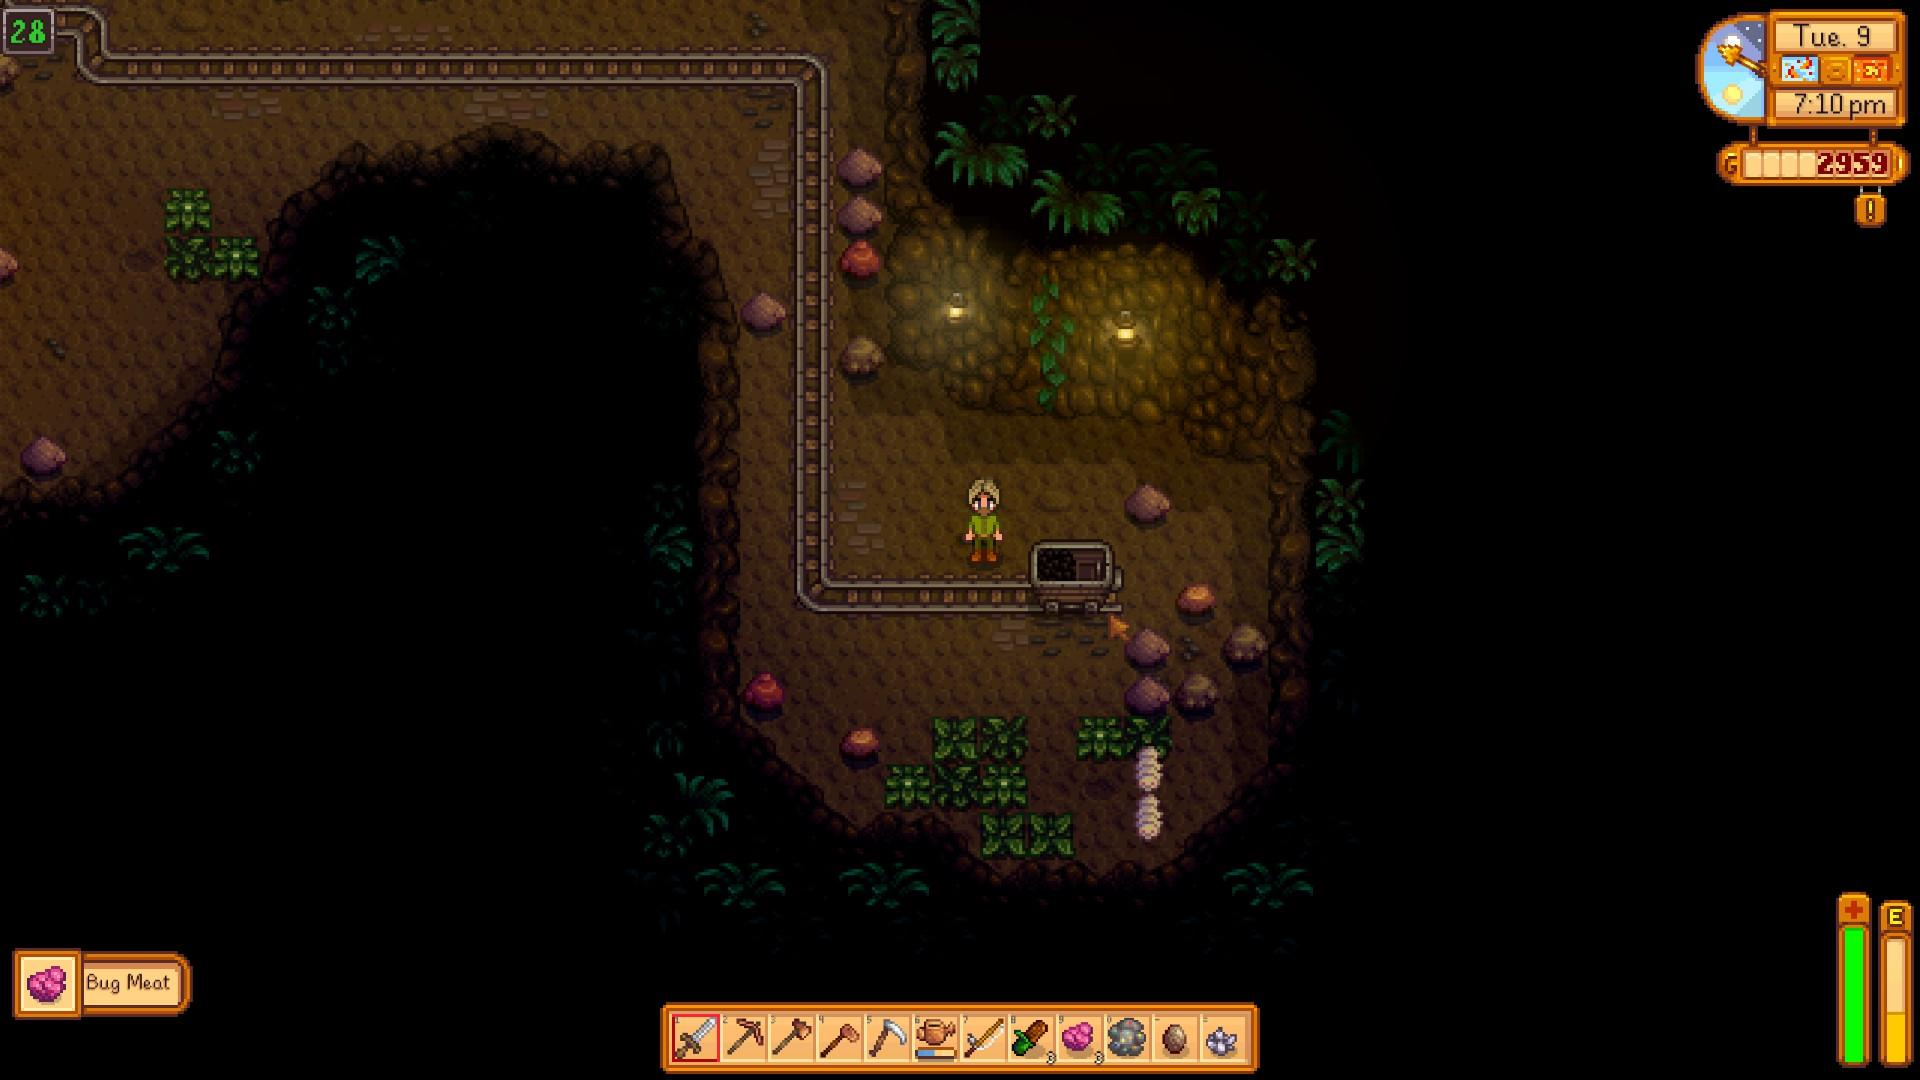
\includegraphics[width=1\textwidth]{StateOfTheArtScreenshots/stardew_valley}
  \label{StateOfTheArt_Screenshots_StardewValley}
  \caption{Screenshot of the game Stardew Valley \cite{StardewValleyScreenshot}}
\end{figure}

Stardew Valley is a 2D top-down indie farming simulation, which features an endless mine, where the player can fight, gather resources for the character and his farm and explore the different levels. The mines consist of an endless amount of procedurally generated levels, with checkpoints after every five levels. These checkpoints can be reached by an elevator on the first level in the mines. Each level consists of several elements, which are mainly gatherable stones and enemies. Furthermore, some levels have special elements, which are quicksand, minecarts, chests, and more. To reach the next level, the player has to find a ladder down, which can be found under a random stone or ore. They can either be destroyed by a pickaxe or bomb. This mine system is only a small part of the overall game but offers a fun and highly replayable experience due to the infinite amounts of levels.

Features:

\begin{itemize}
  \item Top-down rather than a sidescrolling game
  \item Procedurally generated levels
  \item Different themes and enemies for different level regions
  \item Inventory system
  \item Health and energy system
  \item Upgrading of weapons and armor
  \item Resource gathering (for overall game)
  \item Simple 8-bit graphics with customizable character
\end{itemize}

Prices:

\begin{itemize}
  \item Steam: 13.99 EUR
  \item Xbox: 14.99 USD
\end{itemize}
%------------------------------------------------

\subsection{Rogue Legacy}

\begin{figure}[ht]
  \center
  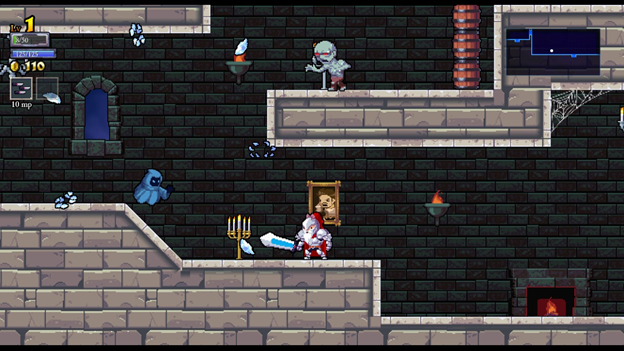
\includegraphics[width=1\textwidth]{StateOfTheArtScreenshots/rogue_legacy}
  \label{StateOfTheArt_Screenshots_RogueLegacy}
  \caption{Screenshot of the game Rogue Legacy \cite{RogueLegacyScreenshot}}
\end{figure}

Rogue Legacy is a 2D game, which was released in 2013 developed by Cellar Door Games. The game has been released for different platforms such as Microsoft Windows, Linux, OS X, PlayStation 3, PlayStation 4, PlayStation Vita and Xbox One \cite{RogueLegacyWiki}. The game is about exploring a randomly generated dungeon and collecting gold. The player(character) has default abilities such as jump and slash with a sword and secondary abilities such as magic attacks by using mana. The player has to defeat a boss in order to go to the next level \cite{RogueLegacyReview}.

Features: \cite{RogueLegacySteam}

\begin{itemize}
  \item Single player
  \item With sword, mana and life gauge to worry about
  \item Traps and obstacles to dodge and avoid
  \item More than 8 classes to choose from
  \item Over 60 different enemies
  \item Powerful weaponry and armor
  \item Tons of secret areas
  \item Boss in every stage
  \item Jump, run and dash
\end{itemize}

Prices:

\begin{itemize}
  \item Steam: 14.99 EUR
  \item Xbox: 13.99 USD
  \item PlayStation: 16.99 USD
\end{itemize}

%------------------------------------------------

\subsection{Mega Miner}

\begin{figure}[ht]
  \center
  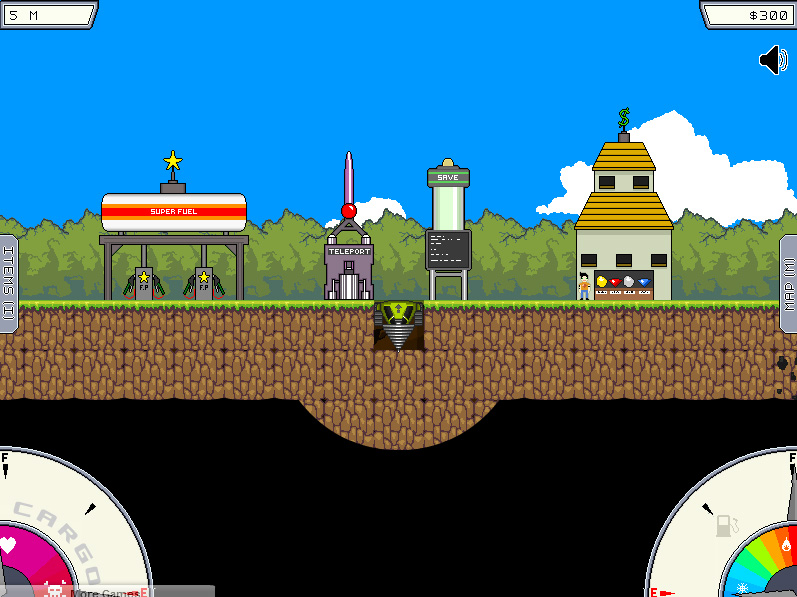
\includegraphics[width=0.8\textwidth]{StateOfTheArtScreenshots/mega_miner}
  \label{StateOfTheArt_Screenshots_MegaMiner}
  \caption{Screenshot of the game Mega Miner \cite{MegaMinerScreenshot}}
\end{figure}

Mega miner is a 2D game developed by Armor Games. The main task in the game is to drill a mine and while this process collects gold, silver, coal and other minerals. Then the player (character) can sell it for cash and upgrade his mining machine by new coolers etc. This game is qualified as a strategy game.

Features:

\begin{itemize}
  \item Single player
  \item Gold, silver, coal and other minerals to collect
  \item Rocks as obstacles to avoid
  \item One map
  \item No enemies
  \item Possibility to upgrade character (drill)
\end{itemize}

Price: Free

%------------------------------------------------

\subsection{Spelunky}

\begin{figure}[ht]
  \center
  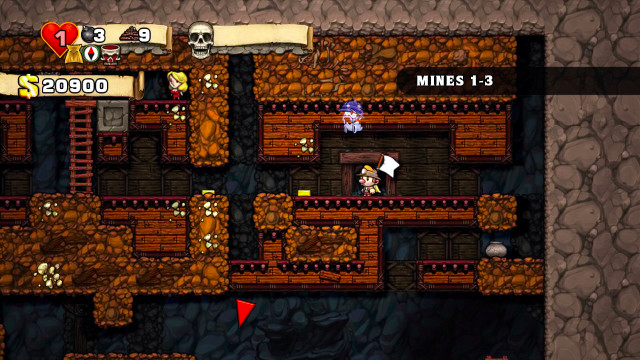
\includegraphics[width=1\textwidth]{StateOfTheArtScreenshots/spelunky}
  \label{StateOfTheArt_Screenshots_Spelunky}
  \caption{Screenshot of the game Spelunky \cite{SpelunkyScreenshot}}
\end{figure}

Spelunky is a 2D cave exploration/treasure-hunting game inspired by classic platform games such as Rayman, Super Mario, and Sonic the Hedgehog. One of the crucial features that differentiate this game to the classic versions, is that the game is top-down rather than sidescrolling, which leaves the player with a completely different feel. With an inventory full of bombs, ropes, and your own whip, the aim is to creatively maneuver through the fully-destructible ancient caves. In order to complete levels, you have to search deep in the underground for a door, while encountering a variety of enemies, as well as traps and treasure. It's a challenging game that will likely test your patience since you will die continuously. But with many deaths comes experience, and eventually, as you beat the level, the frustration is overtaken by a great feeling of satisfaction.

\textbf{Pros and Cons:}

\textbf{Pro:} Skill based gameplay. \emph{In Spelunky the player has everything needed from the start so it is only the skill level of the player that determines whether you advance or not.}

\textbf{Pro:} Roguelike genre allow for quick sessions. \emph{Since the gameplay is so quick, the player will die quite often which means that the sessions tend to be quite short. This makes for a game that can be played in quick bursts throughout the day.}

\textbf{Con:} No check-point system. \emph{You can't save the game and you can't go back to a level with your previous equipment.}

\textbf{Con:} Hard to master. \emph{The game is difficult to the point of frustration.}

Features:

\begin{itemize}
  \item Top-down rather than a sidescrolling game
  \item Skill-based gameplay
  \item Single player and local co-op (up to 4 players)
  \item Traps and enemies to dodge and avoid
  \item Inventory system primarily with bombs and ropes
  \item Money collecting for the shopkeeper in-between levels
  \item Full maneuverability with infinite jumping and running
\end{itemize}

Price: Free

%------------------------------------------------

\subsection{Nuclear Throne}

%------------------------------------------------

\subsection{Conclusion}
Conclusion.

%----------------------------------------------------------------------------------------
%	MARKET ANALYSIS
%----------------------------------------------------------------------------------------

\newpage
\section{Business Strategy} \label{MarketAnalysis}

%----------------------------------------------------------------------------------------

\subsection{Business Model} 
Ever since the release of Pong\cite{Pong} in the U.S. and the beginning of the first generation of video game consoles in 1972 the gaming industry has been growing steadily and sees no end it sight. It has spread throughout the globe and game development companies have become international organisations. The only part of the globe where games are not popular is South America.\cite{GamesMarketRevenue} In the past few years the mobile gaming segment has overtaken all others in revenue and is expected to increase its lead over the coming years.

\begin{figure}[ht]
  \center
  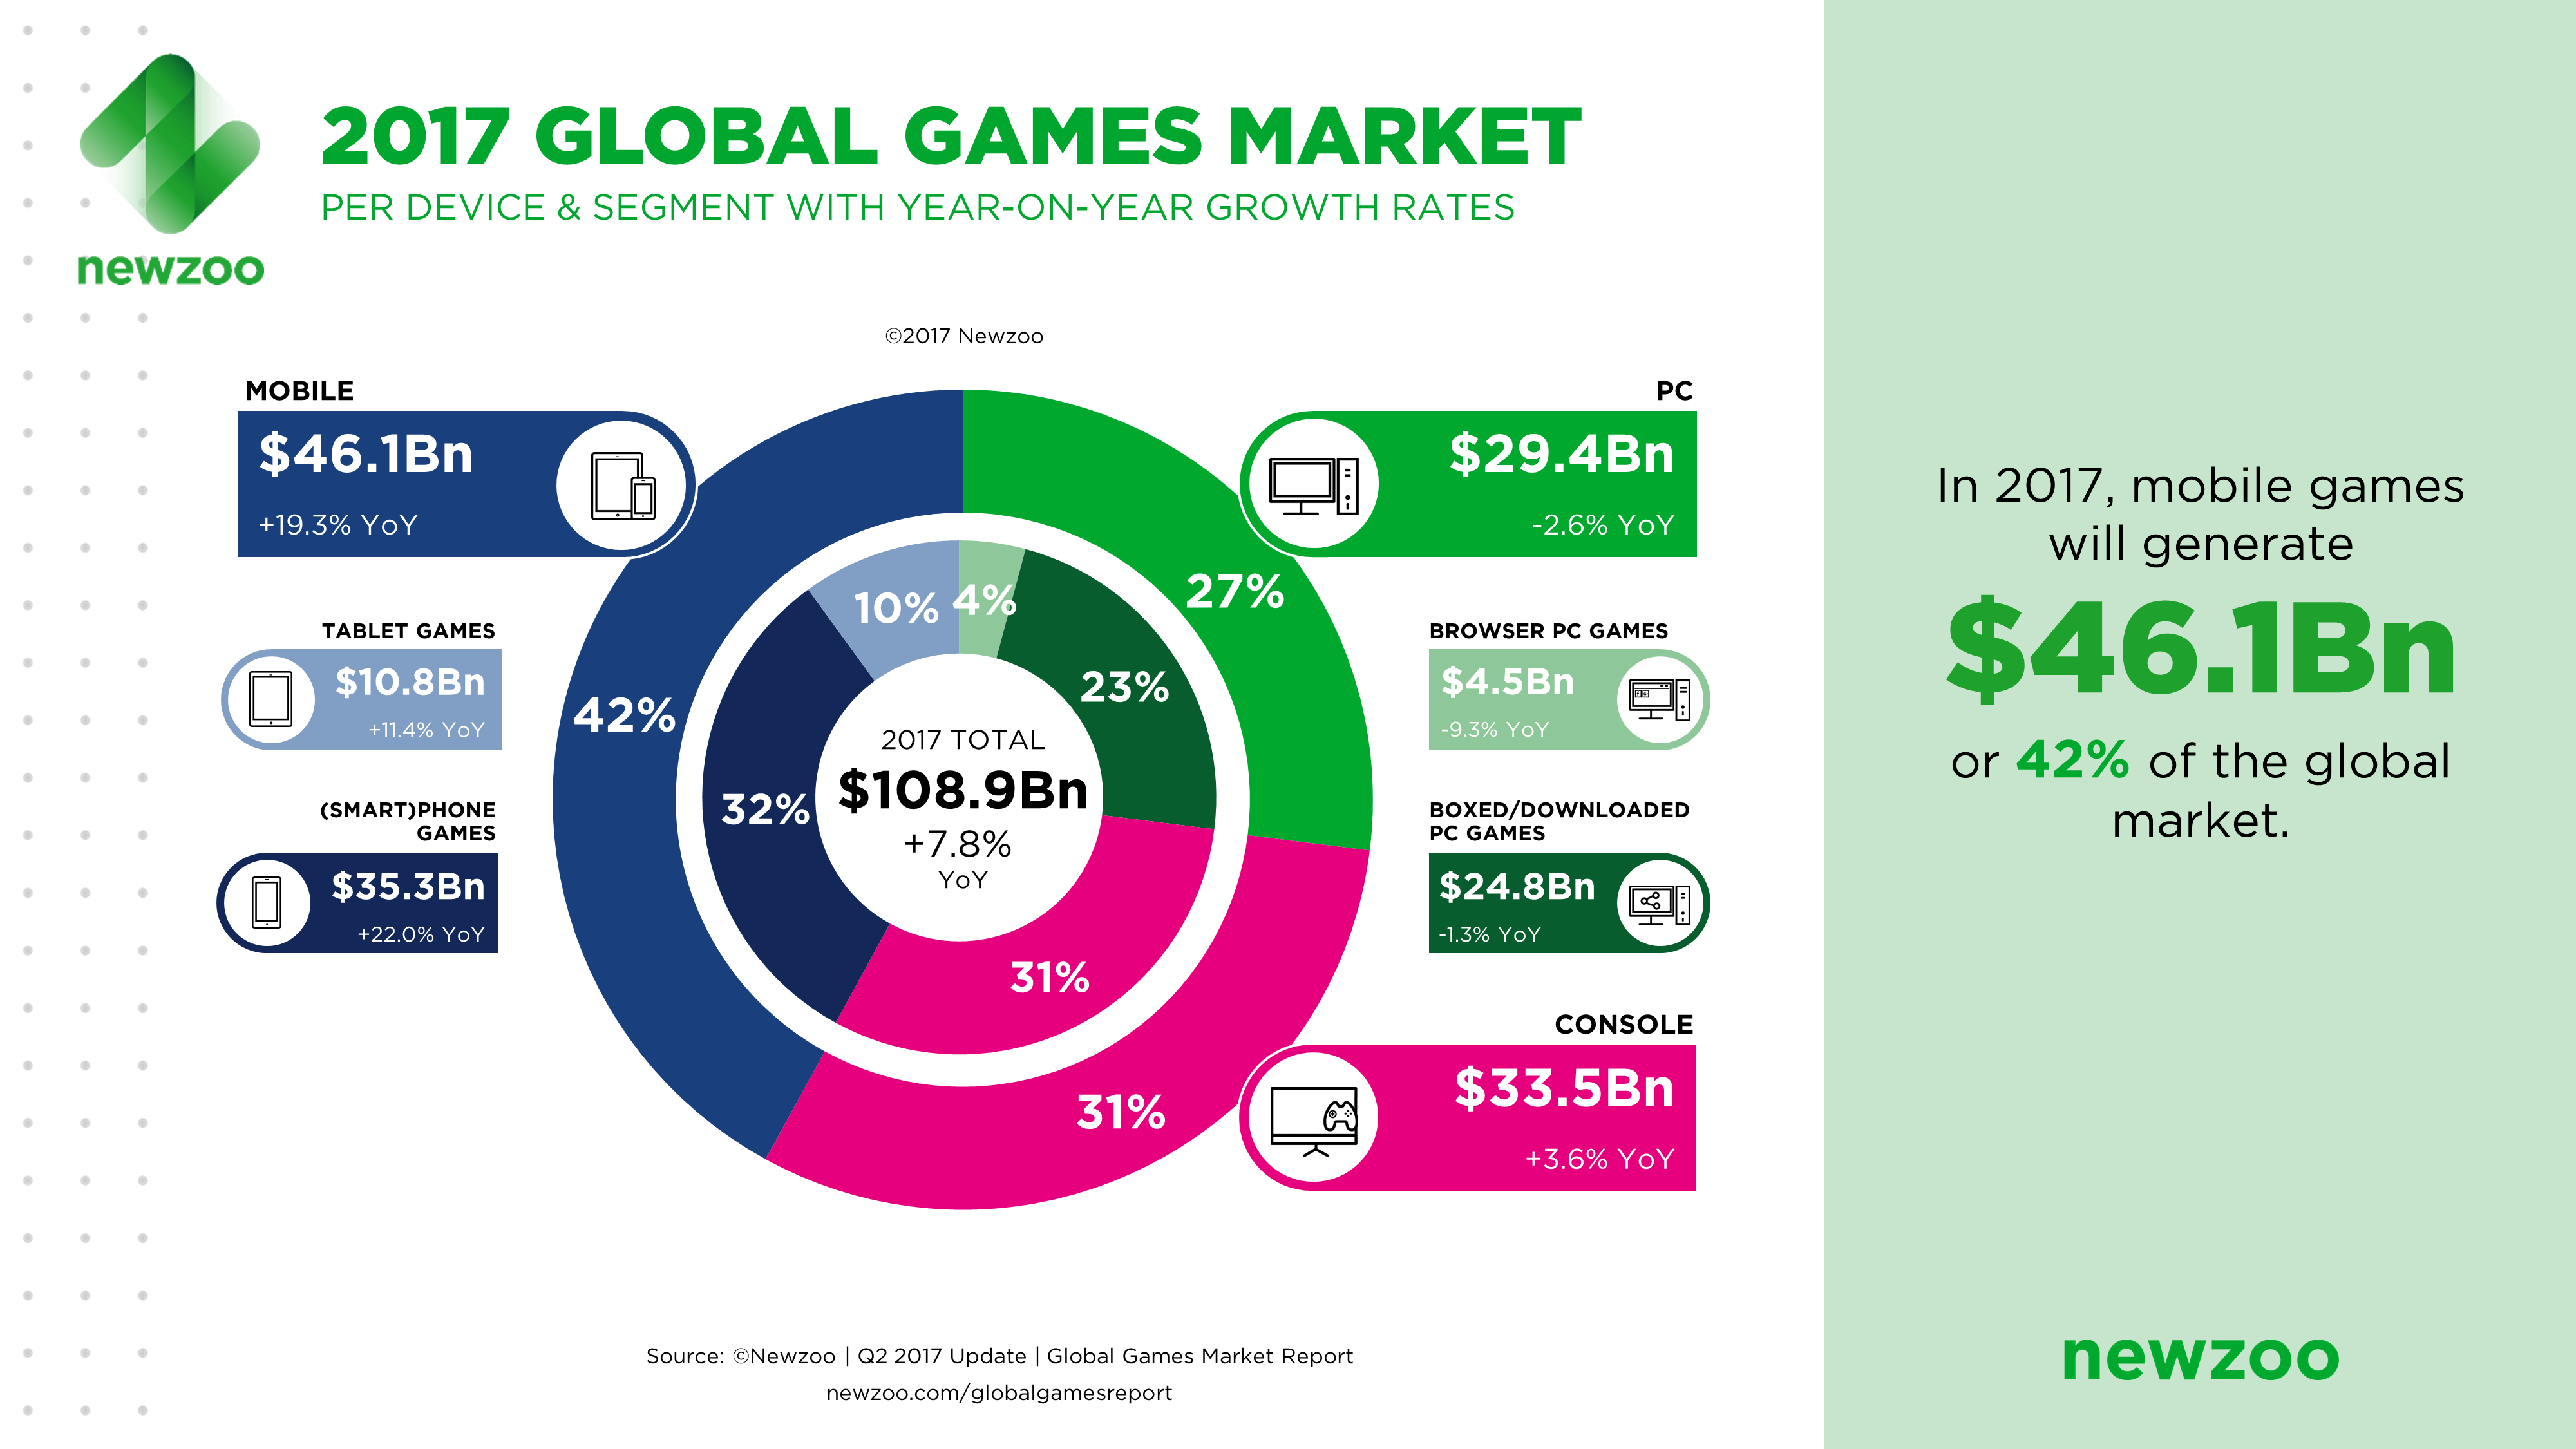
\includegraphics[width=1\textwidth]{BusinessStrategy/Newzoo_2017_Global_Games_Market_Per_Segment_April_2017}
  \label{Newzoo_2017_Global_Games_Market_Per_Segment_April_2017}
  \caption{Newzoo 2017 Global Games Market Per Segment \cite{NezooScreenshot}}
\end{figure}

One of the reasons for this growth is the inclusion of new players - mostly females and elders, has induced the popularity of casual games in social networks and mobile apps. Another is the constant development of the different business models used by game developers. The most successful in recent years has been the free-to-model.\cite{BusinessModelsAndStrategy}

So how to combine these strengths into a model that will help us establish our project in this competitive market?

We plan to use the trends in gaming to our advantage - PC games are still popular, but players expect an impressive gaming experience in return for their money. Mobile games are growing in popularity and lots of people are happy to pay for a simple entertaining experience.

Therefore we plan to release Gangster Squirrel for free for Desktop devices as an effort to boost interest. Mobile versions would be available as well for 1.99\$.

A subscription-based model, though other games have had great success with it, doesn’t make sense in our case, because our game is very short. We plan to build a strong brand with successful sequels of the game, which will help with establishing ourselves in the market.

\subsection{Marketing Strategy}
Through the long history of game development, the marketing utilised by game producers has been quite varied \cite{MarketingStrategyExamples}. Users have been bombarded with promotional videos, print ads, billboards, newsletters and much more. Some companies have benefited from their marketing materials going viral.
Our game will not be distributed on physical media, due to the added cost, it will available solely online. Therefore to aid with the advertisement our marketing will also be online, due to it's high return of investment, analytic capabilities and ease of use.

%	DOCUMENTATION
%----------------------------------------------------------------------------------------

\newpage
\section{Documentation}

%------------------------------------------------

\subsection{Choosing the game engine} \label{DocGameEngine}

Deciding on a game engine is not an easy task, especially for Java. In the group, we split up the research of individual game engines, so that we can gather information about as many as possible before deciding on one. The procedure of finding relevant frameworks and game engines was fairly easy, by searching on a list of game engines on Wikipedia \cite{ListOfGameEngines}, using Google search and reading through forums to determine the public opinion on this topic. It quickly became apparent, that the market is rather thin when it comes to Java-based game engines, the big players like Unity \cite{UnityGameEngine} and Unreal Engine \cite{UnrealEngine} rely on \texttt{C} variations.

We researched the option of using a native Java library like \texttt{JavaFX}, which would imply a lot of work on creating a core foundation for a game since it's not specifically made for this purpose. Most modern game engines come with certain standards, including an already existing application structure (with a game loop, scene management, events, and more). Popular engines usually also include their own or community made tools like map editors, asset managers, user interface composer, physics simulation, and so much more.

All of this would have the consequence of us having to code everything ourselves, limiting the outcome of the project due to the limited time. The group decided against this option by a majority vote. Not having to deal with a lot of very basic problems and therefore being able to develop the game farther and with more features, was more appealing to the majority of the group members.

Moving on, the group settled on a couple of game engines or frameworks to research: \texttt{libGDX} \cite{LibGDX}, \texttt{LWJGL} \cite{LWJGL}, \texttt{jMonkeyEngine} \cite{jMonkeyEngine}, \texttt{mini2Dx} \cite{mini2Dx} and \texttt{Slick2D} \cite{Slick2D}. This selection is mostly by scavenging forum posts and the first page of Google for the search of "Java Game Engines". One particular \emph{Reddit} post \cite{RedditJavaGameEngines} named all of them.

Since \texttt{libGDX} is based on \texttt{LWJGL}, it is easy to compare them. \texttt{LWJGL} is very low-level and doesn't provide many features, compared to \texttt{libGDX}. It is also harder to start off with as a beginner in programming \cite{StackExchangeLibGDXLWJGL}, which is why we went with \texttt{libGDX}. Furthermore, the \texttt{jMonkeyEngine} is mainly developed for 3D applications, which rules it out for our project. 

\texttt{Mini2Dx} and \texttt{Slick2D} are both based on \texttt{LWJGL} too, but considerably smaller than \texttt{libGDX}. Comparing the GitHub pages of libGDX \cite{libgDXGitHub} and mini2Dx \cite{mini2DxGitHub}, this is quickly apparent. \texttt{LibGDX} has more than 400 contributors to the repository, while \texttt{mini2Dx} is only created and maintained by one person when looking at the contributors page. Meanwhile, \texttt{Slick2D} is hosted on BitBucket \cite{Slick2DBitBucket}, and hasn't even created a \emph{Read me} file. Judging from the documentation of the different game engines (can be found on the respective GitHub pages and for \texttt{Slick2D} on their own Wiki page \cite{Slick2DWiki}), it becomes even clearer, which engine is popular and which are not. \texttt{LibGDX} has a very extensive documentation with plenty of examples and in-depth explanations. \texttt{Mini2Dx} has a much smaller documentation, where most topics simply consist of a lot of pasted code without proper explanation. Meanwhile, \texttt{Slick2D}'s wiki page looks almost like an empty wiki template, because there is basically no documentation whatsoever.

This analysis is quite a clear statement, which choice would be the best and most painless way to go, so we decided to go with \texttt{libGDX}.

%------------------------------------------------

\subsection{libGDX Setup} \label{DocSetup}

To set up a libGDX project in IntelliJ IDEA, the official setup tool (see Figure \ref{fig:LibGDXSetupScreenshot}) needs to be used. This creates a Gradle project with all necessary files, adds optional extensions by default and defines the deployment platforms (Windows, macOS, Linux, Android, iOS, Blackberry, and HTML5). By clicking on \emph{Advanced} and selecting IntelliJ IDEA or a different IDE, this tool also creates the project files for the specific IDE.

\begin{figure}[ht]
  \centering
  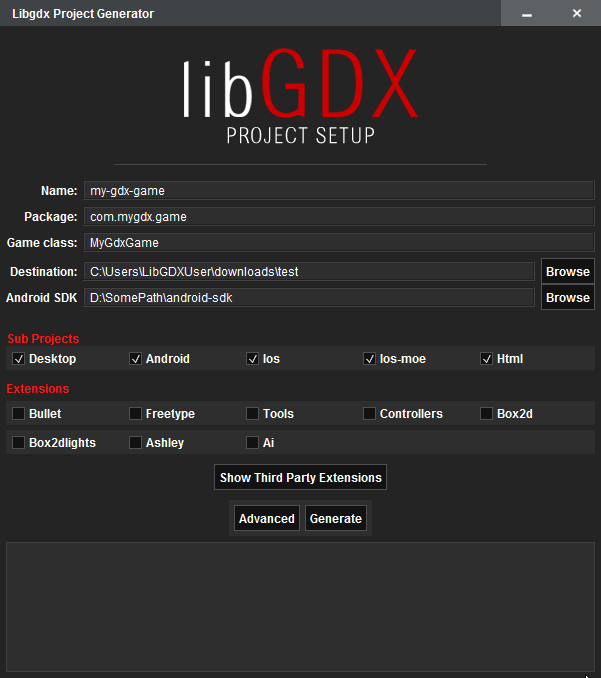
\includegraphics[width=0.6\textwidth]{libGDX_setup.png}
  \caption{libGDX Setup Tool}
  \label{fig:LibGDXSetupScreenshot}
\end{figure}

The import into IntelliJ is easy, just open the project and an import pop-up appears. By simply clicking \texttt{Ok}, everything will be imported and set up and the project is ready. To run the application in a desktop environment, the build configuration needs to be updated first, by setting the working directory to the \texttt{assets} folder of the project. With this being done, the set-up is complete.

%------------------------------------------------

\subsection{The main class} \label{DocMainClass}

Since libGDX applications can run on multiple platforms (Windows, macOS, Linux, Android, iOS, Blackberry, and HTML5), the structure isn't as straightforward as a usual Java application. Considering the project delimitations (see section \ref{ProjectDelimitations}), this project is supposed to only run on the desktop platforms, which is why the focus is there.

Depending on the selected deployment platforms, the project will contain different kinds of \texttt{Launchers}, which handle the execution of the game. All desktop environments run on the same launcher since Java is cross-platform itself. The following code is all it takes to set it up, including setting certain configuration values, which are defined in the main class of the game.

\begin{minted}[linenos,breaklines]{java}
public class DesktopLauncher {
	public static void main (String[] arg) {
		LwjglApplicationConfiguration config = new LwjglApplicationConfiguration();

		config.title = MainGameClass.NAME;
		config.foregroundFPS = MainGameClass.FPS;
		config.width = MainGameClass.WIDTH;
		config.height = MainGameClass.HEIGHT;
		config.fullscreen = MainGameClass.FULLSCREEN;
		config.resizable = MainGameClass.RESIZABLE;

		new LwjglApplication(new MainGameClass(), config);
	}
}
\end{minted}

Going further, the actual code is located in the \texttt{core} directory of the project. Beside that, the generated \texttt{bytecode}, the \texttt{build gradle} file and the \texttt{assets} folder are located here. The assets folder contains all external files, like graphics, fonts and text files, which are used by the game.

The game starts off in the \texttt{MainGameClass}, which runs the very basic foundation of the game, by setting up important public static parameters like screen size, camera settings, gravity, and more. The main class extends libGDX's \emph{abstract} \texttt{Game} class, which itself implements the \texttt{ApplicationListener} \emph{interface}. LibGDX mostly works in an event-driven fashion, which is why there is no game loop \cite{libGDXLifeCycle}. The \texttt{render} method, however, can be considered as such, as it runs every frame. The flowchart in figure \ref{fig:LibGDXLifeCycle} explains the life cycle of a libGDX application quite well.

\begin{figure}[ht]
  \center
  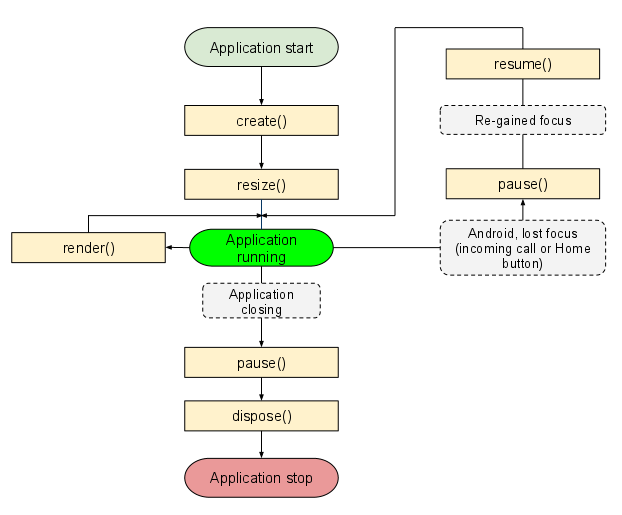
\includegraphics[width=1\textwidth]{Documentation/lifeCycle}
  \caption{LibGDX Life Cycle \cite{libGDXLifeCycle}}
  \label{fig:LibGDXLifeCycle}
\end{figure}

The main class has several purposes. It runs the main game cycle, sets up necessary parameters and has them publicly available to all classes, but also contains some important methods, like resetting certain values in the save files (player lives, current time) and also methods to exit the application. The following code shows the two overloaded exit methods. The difference is simply, that one of them prints out a message before exiting, while the other does not.

\begin{minted}[linenos,breaklines]{java}
public void exitApplication() {
	resetTimer();
	resetPlayerLifes();
	Gdx.app.exit();
	System.exit(0);
}

public void exitApplication(String errorMessage) {
	if (errorMessage != null && !errorMessage.isEmpty()) {
		System.err.println(errorMessage);
	}

	exitApplication();
}
\end{minted}

The methods \texttt{resetTimer()} and \texttt{resetPlayerLifes()} reset the values for the current game time and the current lives of the player in the JSON save files, because they are being used by the game and need to be temporary, or the lives or the time will not start from the default value, when starting the game the next time. These values need to be stored in a file, because the entire play screen class is being reloaded, when the player respawns, and therefore resetting all run time variables.

The game is then being closed by calling the libGDX method \texttt{Gdx.app.exit()}, which disposes of all disposable resources in the application and close the game. This works just fine, but usually prints out a bunch of irrelevant errors, which can be more or less suppressed by calling the native Java method \texttt{System.exit()}. The error code \texttt{0} means the execution went just fine with no errors.

When the main class is done setting things up, including the creation of a new Thread for a connectivity with Twitch (see documentation at \ref{Twitch}), the game switches the \texttt{Screen} to the \texttt{SplashScreen} class, which simply displays a splash screen and then switches to the \texttt{PlayScreen} class, which is the main screen of the game, containing the actual gameplay and manages, how it all comes together. It implements libGDX's \texttt{Screen} class and follows a similar life cycle as described for the main game class.

%------------------------------------------------

\subsection{The application structure} \label{DocApplicationStructure}

As described in the previous section, the \texttt{MainGameClass} is the entry point of the application, followed by the most important class of the game, the \texttt{PlayScreen}. This does not nearly describe the structure of the entire project though since there are dozens of classes in the project.

The following figure \ref{fig:minClassDiagram} is a minimised version of the class diagram of the project, which is supposed to show the relation between classes and the overall structure.

\begin{figure}[ht]
  \centering
  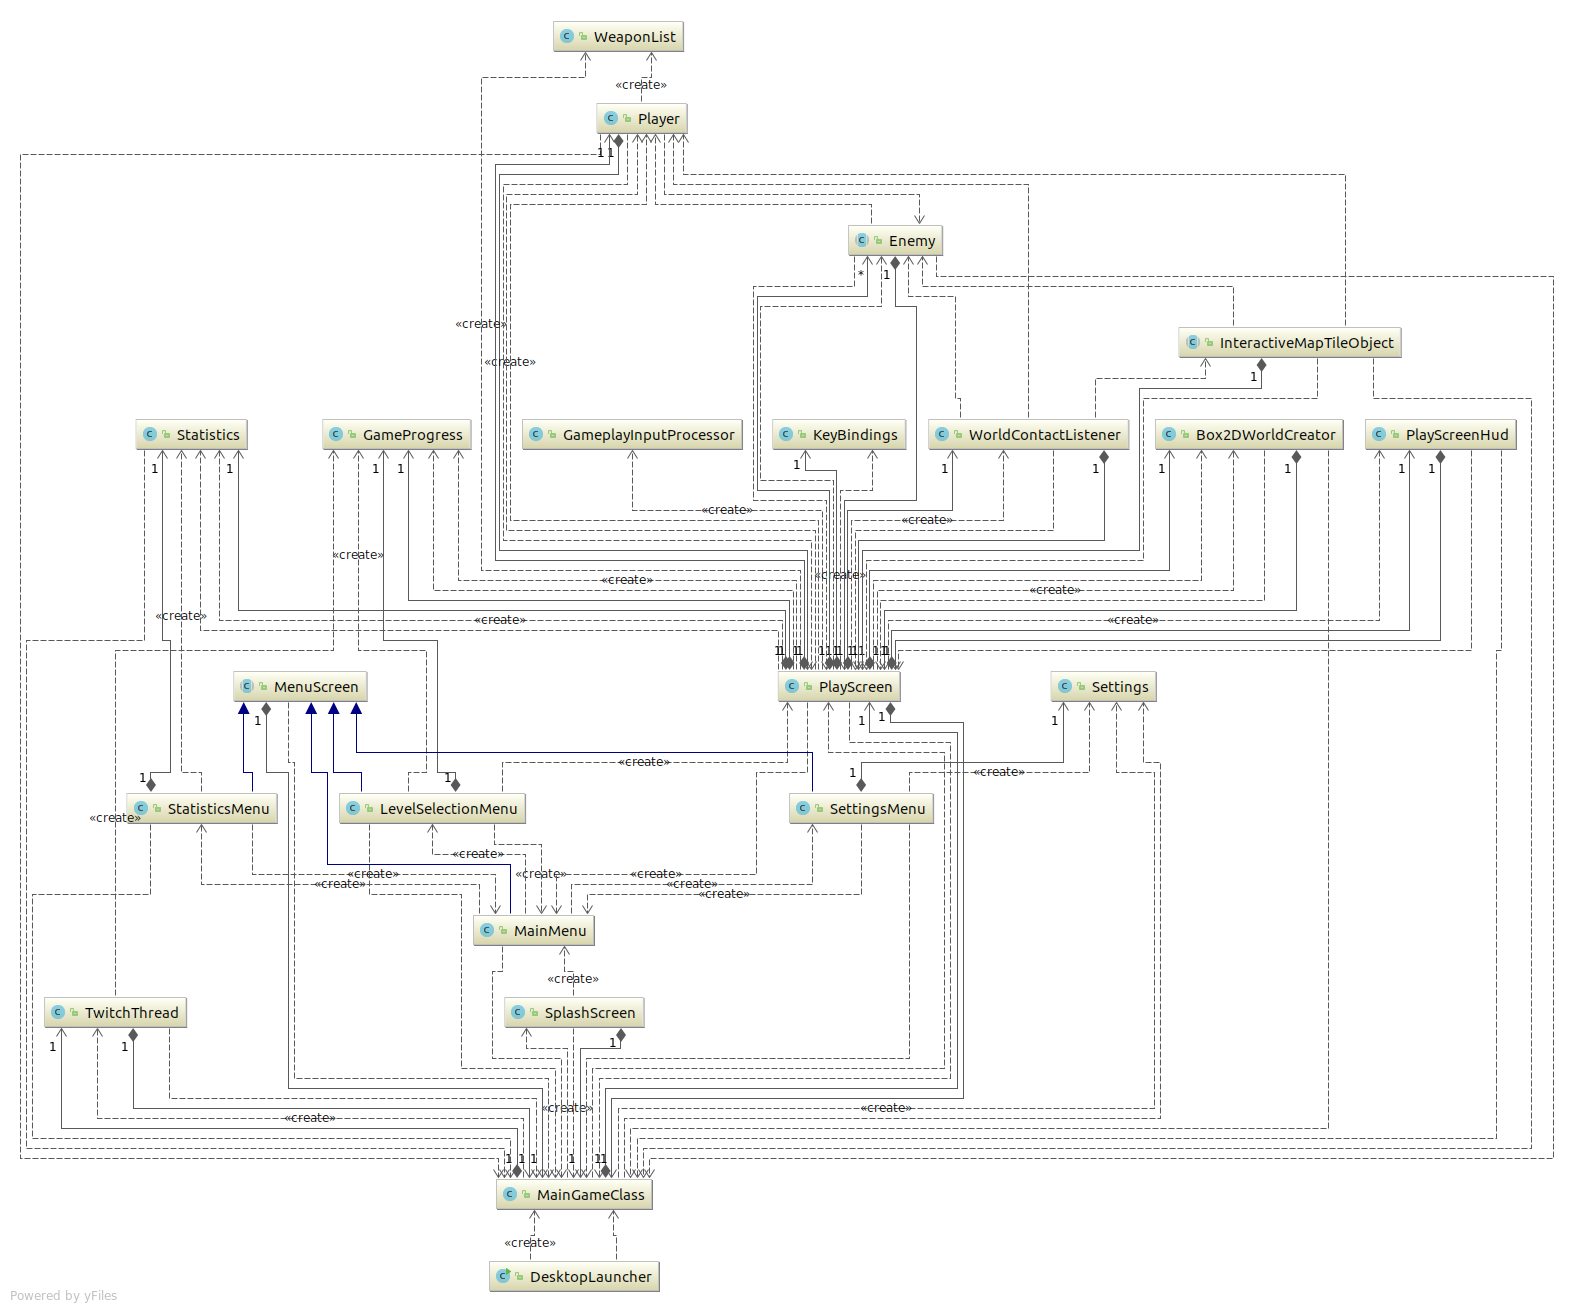
\includegraphics[width=1\textwidth]{Documentation/class_diagram_minimized.png}
  \caption{Minimised class diagram}
  \label{fig:minClassDiagram}
\end{figure}

The application starts with the \texttt{DesktopLauncher}. Other platforms have different launchers, but this project is only available on desktop platforms and is, therefore, the only launcher. The full diagram also shows a \texttt{HtmlLauncher} for running it in a web browser, which is not used, nor supported in our case.

The first actual class of the game is the \texttt{MainGameClass}, which was already explained in the previous section. From there, a separate thread for the Twitch integration is created (see section \ref{Twitch}). The reason, why so many dotted arrows point back to the main class, is because of all the public parameters that are stored here and needed by many classes.

Following that, the main game class creates the \texttt{SplashScreen}, which just shows an image for a few seconds and then switches to the \texttt{PlayScreen}. In here, everything gameplay relevant is being created and handled (see section \ref{DocPlayScreen}). 

The following list briefly describes each class that can be seen in the minimised class diagram, except the ones already described. Many of these classes have subclasses or associated classes, which are not relevant for the structure but can be seen in the full diagram (see section \ref{AppendixClassDiagramFull}).

\begin{itemize}
  \item \textbf{Box2DWorldCreator}: responsible for creating the physics environment of the map (see section \ref{DocPhysicsAndBodySetup} and \ref{DocMaps})
  \item \textbf{WorldContactListener}: detects and handles all collision between physics objects (see section \ref{DocCollisionDetection})
  \item \textbf{InteractiveMapTileObject}: an abstract class for static map objects, includes physical body set up and collision handling (see section \ref{DocPhysicsAndBodySetup})
  \item \textbf{Enemy}: an abstract class for different enemy objects, includes physical body set up, collision handling and enemy movement \textbf{ADD REFERENCE TO SECTION}
  \item \textbf{Player}: the definition of the player as physical entity and as texture. Everything from player animations, moving, attacking and switching weapons is done here \textbf{ADD REFERENCE TO SECTION}
  \item \textbf{PlayScreenHud}: sets up and manages the "Heads Up Display", containing items like the health bar and the timer \textbf{ADD REFERENCE TO SECTION}
  \item \textbf{GameplayInputProcessor}: registers key press events and handles them appropriately (see section \ref{DocKeyBindings})
  \item \textbf{KeyBindings}: reads and writes associated keys with certain actions to a file (see section \ref{DocKeyBindings})
  \item \textbf{GameProgress}: reads and writes the user's progress in the game to a file \textbf{ADD REFERENCE TO SECTION}
  \item \textbf{Statistics}: reads and writes the user's statistics to a file \textbf{ADD REFERENCE TO SECTION}
  \item \textbf{WeaponList}: reads and writes all available weapons in the game to a file \textbf{ADD REFERENCE TO SECTION}
\end{itemize}

%------------------------------------------------
 
\subsection{The Play Screen} \label{DocPlayScreen}
 
%------------------------------------------------

\subsection{Physics and collision detection} \label{DocCollisions}

One of the most important aspects of a game is certainly the collision detection and handling between objects. Without it, it would not be possible to even make the player walk on a flat surface.

LibGDX utilizes \texttt{Box2D}, a famous physics engine for rigid body simulations, originally written in \texttt{C++} and since ported into many other languages. It was used in several well known games like \emph{Angry Birds}, \emph{Tiny Wings}, \emph{Limbo}, and \emph{Happy Wheels} \cite{box2DGithub}\cite{box2DWikipedia}.

\subsubsection{Physics and map objects setup} \label{DocPhysicsAndBodySetup}

As described in the map documentation (see section \ref{DocMaps}), the maps that are created in the \texttt{Tiled} map editor, can contain so-called object layers, which contain information about shapes, that will be used as collision shapes in the game. For example, when creating a simple two-dimensional map in a map editor, you obviously add graphics. The game can't know, what the world actually looks like just by the textures though. It needs concrete information on what to treat as walkable ground, what enemies are, where a finish line might be, and so on. This is where the object layers come into play.

Before we can go on to detecting collisions and handling them, we obviously first need to create a world and all it's bodies, in order to play with them. The first step towards this is done in the \texttt{PlayScreen} class within the constructor. Here, a \texttt{World} object is created, which contains all bodies and controls the entire physics simulation. The following line of code initializes the world, with the parameter of the gravity, which is roughly $9.81m/s^2$ in the negative direction of the Y-axis. This value is a final floating point value, defined in the main game class amongst the other constant values. The second parameter, \texttt{doSleep}, improves the performance of the simulation if set to \texttt{true}, by not simulating inactive bodies, which means bodies that do not move or interact in any other way with the world, at the specific time.

\mint{java}{world = new World(new Vector2(0, - MainGameClass.GRAVITY), true);}

Furthermore, a \texttt{Box2DWorldCreator} and \texttt{WorldContactListener} class are initialized in the same constructor. Both of them are custom written classes, the first one being responsible for reading the shapes from the map file and translating them into actual bodies in the world. This is partially described in the maps documentation in section \ref{DocMaps}. The second class implements libGDX's \texttt{ContactListener} class and constantly listens for collisions between objects and calls the required methods. This is documented in the next section (\ref{DocCollisionDetection}).

All static objects in the map are child objects of the abstract \texttt{InteractiveMapTileObject} class, which defines a standard structure for these objects. Since all objects in the map have a rectangular shape, this abstract class implements a standardized way of setting up the body of each object. All it needs to know is the rectangle, which defines shape and position of the object, and if it is a sensor. If an object is a sensor, collisions will be detected as usual, but other objects can't collide with it visually and will simply move through them. This can be useful for many different purposes, for example, the weapon pick-up mechanics.

As an example, we take the \texttt{DeathTile} class and follow it's steps to creation. This type of object has the purpose of killing both players and enemies if they come in contact with it. This will often be graphically represented by spikes. As described in section \ref{DocMaps}, for each object in an object layer, the program creates an instance of the related child class of an \texttt{InteractiveMapTileObject}. In this case, a \texttt{DeathTile}. The object will then be added to a list, which contains all objects of this type.

\mint{java}{deathTileObjects.add(new DeathTile(screen, rectangle));}

The constructor demands the \texttt{PlayScreen} object as the first parameter, so it has access to it. The second parameter is the rectangle that was read from the map file.

The following code snippet is from the \texttt{DeathTile} class in order to explain the creation of such objects.

\begin{minted}[linenos,breaklines]{java}
public class DeathTile extends InteractiveMapTileObject {

    private PlayScreen playScreen;

    public DeathTile(PlayScreen screen, Rectangle bounds) {
        super(screen, bounds, true);
        this.playScreen = screen;

        fixture.setUserData(this);
        createFilterMask();
    }

    @Override
    public void onPlayerBeginContact(Player player) {
        playScreen.setPlayerCurrentHealth(-1);
    }

    @Override
    public void onPlayerEndContact(Player player) { }

    @Override
    public void onEnemyBeginContact(Enemy enemy) {
        enemy.setHealth(-1);
    }

    @Override
    public void onEnemyEndContact(Enemy enemy) { }

    @Override
    public void createFilterMask() {
        Filter filter = new Filter();
        filter.categoryBits = MainGameClass.CATEGORY_DEATHTILE;
        filter.maskBits = MainGameClass.MASK_DEATHTILE;
        fixture.setFilterData(filter);
    }
}
\end{minted}

In the constructor, the \texttt{super} method is called, which is the constructor of the InteractiveMapTileObject, which handles the physics setup. In addition to the \texttt{PlayScreen} and the rectangle, a boolean variable is passed as a parameter. It defines, if the object is a sensor, as described above.

Still in the constructor, the \texttt{User Data} of the \texttt{fixture} is set to the class itself, \texttt{this}. The \texttt{fixture} is a \texttt{protected} variable of the parent class and therefore available in the child class scope. The \texttt{User Data} is a value that is important for collision detection. It can be any \texttt{Object} and will later be used to identify a collided object, as described in section \ref{DocCollisionDetection}.

The method \texttt{createFilterMask} is an abstract method of the parent class, that each child has to implement. It sets up collision filtering, which is also described in section \ref{DocCollisionDetection}.

The four remaining abstract methods are always called, when either a player or enemy is colliding with this specific \texttt{DeathTile} object. In this case, when a contact begins, the health of either of those will be set to $-1$, which kills them in the next frame.

The last code snippet for this section finally shows, how a map object is actually created. The code is from the \texttt{InteractiveMapTileObject} class. Besides the shown constructor, the class defines the five abstract methods and contains two methods that are used for picking up weapons (see section \ref{DocWeaponCollection}).

\begin{minted}[linenos,breaklines]{java}
public InteractiveMapTileObject(PlayScreen screen, Rectangle bounds, boolean isSensor) {
        this.playScreen = screen;
        this.world = screen.getWorld();
        this.map = screen.getMap();
        this.bounds = bounds;

        BodyDef bodyDef = new BodyDef();
        FixtureDef fixtureDef = new FixtureDef();
        PolygonShape shape = new PolygonShape();

        bodyDef.type = BodyDef.BodyType.StaticBody;
        bodyDef.position.set((bounds.getX() + bounds.getWidth() / 2) / MainGameClass.PPM, (bounds.getY() + bounds.getHeight() / 2) / MainGameClass.PPM);
        body = world.createBody(bodyDef);

        shape.setAsBox(bounds.getWidth() / 2 / MainGameClass.PPM, bounds.getHeight() / 2 / MainGameClass.PPM);
        fixtureDef.shape = shape;
        fixtureDef.isSensor = isSensor;
        fixture = body.createFixture(fixtureDef);
    }
\end{minted}

In here, the body of the map object is defined with the help of a \texttt{body definition}, \texttt{fixture definition} and \texttt{polygon shape}. The type of the body is \texttt{static} since the map objects should not move upon contact with another object like the player and enemies do (they are \texttt{dynamic}). The position of the body is then being set to the middle of the rectangle. \texttt{bounds.getX()} and \texttt{bounds.getY()} return the lower left corner of the object, which is why half of the width and height is added. This value is then being divided by the \texttt{pixels per meter} scaling unit, which \texttt{Box2D} needs since it's never a good idea to code in pixels. A clarification can be found in a great Stackoverflow answer \cite{stackoverflowPPM}. The shape is then set to a box, with the width and height of the rectangle. The values are divided into two because the \texttt{setAsBox} method takes in the radius of a box.

%------------------------------------------------

\subsubsection{Collision detection} \label{DocCollisionDetection}

In order to detect and handle collisions, libGDX provides a \texttt{ContactListener} interface, that we can use to process all collisions in the world. It is event-driven, which means the methods \texttt{beginContact} and \texttt{endContact} will only be triggered, when a collision happens, not each frame. You then get a \texttt{Contact} object, which manages two colliding shapes and gives the program information about them.

The contact listener is simply attached to the \texttt{Box2D} world in the \texttt{PlayScreen}:

\begin{minted}[linenos,breaklines]{java}
worldContactListener = new WorldContactListener(this);
world.setContactListener(worldContactListener);
\end{minted}

The following code snippet is from the \texttt{WorldContactListener} class and shows the collision handling for player contacts. The code for enemy collisions is very similar and can be found in the source code. To keep it short, the collision between player and enemies is also cut out.

\begin{minted}[linenos,breaklines]{java}
private void processContact(Contact contact, boolean beginOrEndContact) {

        Fixture fixtureA = contact.getFixtureA();
        Fixture fixtureB = contact.getFixtureB();

        if (fixtureA.getUserData() instanceof Player || fixtureB.getUserData() instanceof Player) {
            Fixture player = fixtureA.getUserData() instanceof Player ? fixtureA : fixtureB;
            Fixture collidedObject = player == fixtureA ? fixtureB : fixtureA;

            if (collidedObject.getUserData() instanceof InteractiveMapTileObject) {
                if (beginOrEndContact) {
                    ((InteractiveMapTileObject) collidedObject.getUserData()).onPlayerBeginContact((Player) player.getUserData());
                } else {
                    ((InteractiveMapTileObject) collidedObject.getUserData()).onPlayerEndContact((Player) player.getUserData());
                }
            }
        }
    }
\end{minted}

The method \texttt{processContact} is called from \texttt{beginContact} and \texttt{endContact}, passing a boolean as a parameter, to determine from what method it was called. This is done to avoid having almost identical code twice.

The \texttt{contact} object provides the collided fixtures, which give information about the objects, including the \texttt{user data}, that was mentioned in section \ref{DocPhysicsAndBodySetup}. Since the user data is simply the class itself for map objects and also players and enemies, we can determine the type of object with the \texttt{instanceof} operator. In the first \texttt{if} statement, the operator returns true, if either of the collided fixtures is an instance of the \texttt{Player} class. By this, we can determine if the detected collision is at all related to the player.

Going further, two new fixtures are created that simply store either fixture A or B. This is done to definitely know, which fixture is the player and which is the object the player collided with. The player fixture is assigned by checking, which of the two fixtures is an instance of the \texttt{Player} class. The collided object fixture is then simply the other one.

After determining that, the collided object fixture is tested if it is an instance of the InteractiveMapTileObject class. If this is the case, the relevant method of the map object class is called, giving in the \texttt{Player} object, so the method can work with it. These methods are described in the previous section \ref{DocPhysicsAndBodySetup}.

%------------------------------------------------

\subsubsection{Collision filtering}

Not all objects in the world should be able to collide with all other objects. These unwanted cases can be, of course, just be ignored in the \texttt{Contact Listener}. However, libGDX provides a neat way to create filters for each type of object.

Each type of object is assigned a unique number. After that, filters for each object are created by combining the numbers of the objects that are wanted to collide with this specific object, into one single number. The fixture of each object type will then be assigned the unique number as the \texttt{category bits} and the filter number as the \texttt{mask bits}.

To make this work, these unique numbers need to follow a certain pattern, or else it will not be possible to accurately determine, what numbers contributed to the merged number that is used as the \texttt{mask}.

The pattern is a simple geometric sequence with the factor of two ($1, 2, 4, 8, 16, ...$). The numbers are stored in a 16-bit \texttt{short}, which has a maximum value of $32,767$. Representing these numbers in binary 16-bit notation, they look like this:

\begin{itemize}[leftmargin=*]
    \itemsep-0.75em 
    \item[] $000000000000000\mathbf{1}$
    \item[] $00000000000000\mathbf{1}0$
    \item[] $0000000000000\mathbf{1}00$
    \item[] $000000000000\mathbf{1}000$
    \item[] $00000000000\mathbf{1}0000$
    \item[] $...$
\end{itemize}

Using the \texttt{inclusive bitwise OR} operator \cite{bitwiseOROperator} of Java, we can combine these numbers into one.

The following code snippet shows the definition of all the category bits in the project. They are defined in hexadecimal values (\texttt{0x}) for readability, it doesn't matter if they are written in binary (\texttt{0b}), hexadecimal or decimal. The hexadecimal notation simply allows putting zeros in front, which makes it more readable.

\begin{minted}[linenos,breaklines]{java}
public static final short CATEGORY_PLAYER               = 0x0001;
public static final short CATEGORY_ENEMY                = 0x0002;
public static final short CATEGORY_GROUND               = 0x0004;
public static final short CATEGORY_DEATHTILE            = 0x0008;
public static final short CATEGORY_WEAPON               = 0x0016;
public static final short CATEGORY_FINISH               = 0x0032;
public static final short CATEGORY_JUMPABLE             = 0x0064;
public static final short CATEGORY_ENEMY_MOVE_BORDER    = 0x0128;
public static final short CATEGORY_PLAYER_ATTACK        = 0x0256;
\end{minted}

The following example now shows the creation of the mask bits for the player, which determines what he can collide with.

\begin{minted}[linenos,breaklines]{java}
public static final short MASK_PLAYER = CATEGORY_ENEMY | CATEGORY_GROUND | CATEGORY_DEATHTILE | CATEGORY_WEAPON | CATEGORY_FINISH | CATEGORY_JUMPABLE;
\end{minted}

The \texttt{inclusive bitwise OR} operator now takes all the numbers that are in the statement above and compare them bit for bit. If any of these numbers contain a $1$ at the bit position, the result will also have a $1$ at that position. If none of them do, the result will have a $0$ at that position. Since all numbers only have one single bit where the value is a $1$, each bit in the final result represents one category and if it is contained in that mask or not.

Taking all variables into consideration, the result of the above assignment to the mask of the player will look like that: $00\mathbf{111111}0$

Or in 16-bit notation: $000000000\mathbf{111111}0$

We can now assign a category and the corresponding mask to an object type, which was briefly mentioned in the previous section \ref{DocPhysicsAndBodySetup}.

\begin{minted}[linenos,breaklines]{java}
playerFixtureDef.filter.categoryBits = MainGameClass.CATEGORY_PLAYER;
playerFixtureDef.filter.maskBits = MainGameClass.MASK_PLAYER;
\end{minted}

The \texttt{Contact Listener} will now only take objects into consideration, that have matching filter masks. For example, collisions between an enemy and the finish line, weapon pickups, and more will simply be ignored.

%------------------------------------------------

\subsection{Using key bindings for player input} \label{DocKeyBindings}

Key bindings in games are used to give the players the possibility to individually adjust their setup as they like. Players might want to change the assigned keys for certain actions in the game, if they have unusual keyboard layouts, use other types of input devices like gamepads, or simply like to change a certain key. This gives more flexibility since hard-coded keys can cause frustration and cause an unfavourable opinion about the game.

LibGDX has two different kinds of input processing, the first one being the \texttt{Input} class included in the framework, which uses polling to get key presses. The second method is using an \texttt{InputProcessor}, also included in the framework, which uses events to control input. The key difference between those is, that one can check if a specific key is being pressed at the time of checking with the polling method. An input processor, however, triggers events when certain input events happen, like pressing down a key and then delivering the key code of the pressed key. This allows the input management to be more "clean" and efficient since one can't easily check if one of many flexible keys is being pressed without an input processor.

In order to change and save key bindings, there needs to be a data structure. This is represented in the \texttt{KeyBindingObject} class. One object each represents a single action in the game, represented by a String, and an array of integers, which represent the codes of the keys that are assigned to this action. Therefore, multiple keys can be assigned to one action.

Furthermore, the game has to save this information in a file to make it persistent, or the information will be lost once the application is closed. Therefore, the game will save and load the key bindings into a JSON (JavaScript Object Notation) file, which is a standard data interchange format. Handling this operation is done by the \texttt{KeyBindings} class. 

This class has public lists of the type Integer, which store the key codes for each individual action. These lists are read by the game to process input. In the constructor of the class, the program searches for the JSON file and if it exists, it reads it with the help of \texttt{GSON} \cite{GSON}, an open-source library by Google to convert Java Objects into JSON strings and back. If the file doesn't exist or is empty, a new one will be created and the default keys will be assigned to each action by writing them to the new file and then read them again. Those default keys are hardcoded in the constructor as a \texttt{KeyBindingObject} array.

However, if the file does exist, the JSON string is read from it and converted to an array of \texttt{KeyBindingObject}'s. Each key object will then be assigned to the proper list, that was mentioned earlier. This is done by looping through each object and adding it to the lists by comparing the String attribute, described as \texttt{}{action}. This procedure is called deserialization and can be seen in the \texttt{deserializeKeyBindings()} method of the \texttt{KeyBindings} class.

An exemplary key bindings JSON key binding file looks like this:
\inputminted[linenos,breaklines]{json}{code/json/keybindings.json}

An array in JSON starts with a \texttt{[}, hence the bracket at the start and end. The \texttt{KeyBindingObject} objects in between are items of that array. Each item has a String identifier and another array for the corresponding key codes. JSON separates key and value with a \texttt{:} symbol.

As described earlier, the game uses an \texttt{InputProcessor} to handle gameplay relevant input. Since the game has to recognize when a key is pressed, and not just fire an event once a key is pressed down once, it uses public booleans to toggle between an action being active or not. Otherwise, the player would get a move impulse, for example, only once instead of for the duration of the key press. This logic is located in the \texttt{GameplayInputProcessor} class. When a key is being pressed down or being released, it checks, if the key code of the pressed key is in one of the lists. If that is the case, the \texttt{boolean} is toggled. This \texttt{boolean} is a member of the \texttt{PlayScreen} class and is \texttt{public static} to be available in this class, and is being imported in a static context, hence the missing class reference in the Input Processor class.

Finally, all of this is then used in the \texttt{update} loop of the \texttt{PlayScreen}, which is executed each frame. This is an example of the movement in the right direction:

\begin{minted}[linenos,breaklines]{java}
if (isPressingMoveRight &&
  player.body.getLinearVelocity().x <= player.getMaxWalkVelocity()) 
{
  player.body.applyLinearImpulse(new Vector2(player.getWalkImpulseVelocity(), 0), player.body.getWorldCenter(), true);
}
\end{minted}

Here, it is simply being checked, if the user presses a key that is associated with the action of moving in the right direction, by evaluating \texttt{isPressingMoveRight}. If this is the case, a linear impulse in the right direction is being applied to the player.

 %------------------------------------------------

\subsection{Visual Documentation} \label{DocVisual}

 %------------------------------------------------

\subsection{Tech Documentation} \label{DocTech}

 %------------------------------------------------

\subsection{Animations} \label{DocAnimations}

An animation can be described as the illusion of movement caused by rapidly switching between different static images. We animated our characters by using libGdx's Animation Class \cite{libGdxAnimClass}. An animation consists of multiple frames which are shown in a sequence at set intervals. The Animation Class stores a list of objects representing the sequence. Each object in the Animation is called a keyframe, and multiple keyframes make up the animation.

A typical 2D animation consists of a number of TextureRegions and would be specified as:

\mint{java}{Animation<TextureRegion> myAnimation = new Animation<TextureRegion>(...);}

Every animation needs a sprite sheet - that's an image consisting of all the frames for the animation.

\begin{figure}[ht]
  \center
  
\includegraphics[width=1\textwidth]{Documentation/frog.jpg}
  \caption{Sprite Sheet Example}
  \label{SpriteSheetExample}
\end{figure}

The sprite sheet contains two different animations - the first 4 frames from left to right are used to animate movement. The last 4 are used for the attack animation. To help select the correct parts of the sprite sheet while animating, a TextureAtlas is generated. Among other information about the sheet, it contains the start position of the two types of animation (lines 6 and 13). Here is an example:

\begin{minted}[linenos,breaklines]{text}
frog.png
size: 256, 32
format: RGBA8888
filter: Nearest,Nearest
repeat: none
frog_jump
 rotate: false
 xy: 0, 0
 size: 128, 32
 orig: 128, 32
 offset: 0, 0
 index: -1
frog_attack
 rotate: false
 xy: 128, 0
 size: 128, 32
 orig: 128, 32
 offset: 0, 0
 index: -1
\end{minted}

All the texture atlases are defined in the game's \texttt{PlayScreen} class, using the following syntax:

\begin{minted}[linenos,breaklines]{java}
//Define frog atlas
enemyFrogTextureAtlas = new TextureAtlas("sprites/enemies/frog/frog.atlas");

//Frog atlas getter
public TextureAtlas getEnemyFrogTextureAtlas() {
  return enemyFrogTextureAtlas;
}
\end{minted}

The defined atlases can be reached from other classes via a getter.

We created the actual animations in the class for each specific character. 

The first step is to add all the frames we'll need into an array, by selecting the start of the animation from the texture atlas and iterating until we have collected all the frames (in this case the frames are 4).

The second step is to pass the speed of the animation to the Animation Class along with the animation frames.

\begin{minted}[linenos,breaklines]{java}
//Define jump animation
jumpFrames = new Array<>();
for(int i = 0; i < 4; i++) {
  jumpFrames.add(new TextureRegion(
    screen.getEnemyFrogTextureAtlas().findRegion("frog_jump"), i * ENEMY_PIXEL_WIDTH, 0, ENEMY_PIXEL_WIDTH, ENEMY_PIXEL_HEIGHT)
  );
}
jumpAnimation = new Animation<>(0.4f, jumpFrames);
\end{minted}

It's up to the developer though to specify when and for how long the animation is run. In our case, we jump animation is in a continuous loop, and the attack is used only when the enemy and player are in contact.

\begin{minted}[linenos,breaklines]{java}
public void update(float deltaTime) {
  setRegion(jumpAnimation.getKeyFrame(stateTime, true));
}
\end{minted}

%------------------------------------------------

\subsection{Weapon collecting} \label{DocWeaponCollection}

When they player comes in contact with a weapon the item is added to the player's weapon collection. The logic behind that feature has been implemented in the \texttt{WeaponPickup} class. Every time the played collides with an enemy, the \texttt{onPlayerBeginContact} method is called, which detects what kind of weapon the player has picked up and adds it to the weapon's list if it is not already present. The weapon type is setup in the map. After the item is picked up, it is removed from the map.

\begin{minted}[linenos,breaklines]{java}
 public void onPlayerBeginContact(Player player) {
    // Remove texture
    getCell(map.getLayers().getIndex("graphics")).setTile(null);

    // Add the picked up weapon
    MapObject pickedUpWeapon = getCollidingMapObject(map.getLayers().getIndex("weapon"));
    if (pickedUpWeapon != null && pickedUpWeapon.getProperties().containsKey("weapon_name")) {
      String weaponName = pickedUpWeapon.getProperties().get("weapon_name", String.class);
      playScreen.log("Picked up weapon: " + weaponName);

      boolean changedWeaponList = false;
      ArrayList<WeaponObject> playerWeaponList = playScreen.getPlayer().getWeapons();
      WeaponObject weapon;
      
      switch (weaponName) {
        case "Fists":
          weapon = getWeaponObjectByName("Fists");
          if (weapon != null && !weaponAlreadyInList(weapon)) {
            playerWeaponList.add(weapon);
            changedWeaponList = true;
          }
          break;
        case "Branch":
          weapon = getWeaponObjectByName("Branch");
          if (weapon != null && !weaponAlreadyInList(weapon)) {
            playerWeaponList.add(weapon);
            changedWeaponList = true;
          }
          break;
        case "Swiss Army Knife":
          weapon = getWeaponObjectByName("Swiss Army Knife");
          if (weapon != null && !weaponAlreadyInList(weapon)) {
            playerWeaponList.add(weapon);
            changedWeaponList = true;
          }
          break;
        case "Switchblade":
          weapon = getWeaponObjectByName("Switchblade");
          if (weapon != null && !weaponAlreadyInList(weapon)) {
            playerWeaponList.add(weapon);
            changedWeaponList = true;
          }
          break;
        case "Katana":
          weapon = getWeaponObjectByName("Katana");
          if (weapon != null && !weaponAlreadyInList(weapon)) {
            playerWeaponList.add(weapon);
            changedWeaponList = true;
          }
          break;
        case "Tommy Gun":
          weapon = getWeaponObjectByName("Tommy Gun");
          if (weapon != null && !weaponAlreadyInList(weapon)) {
            playerWeaponList.add(weapon);
            changedWeaponList = true;
          }
          break;
        case "Bazooka":
          weapon = getWeaponObjectByName("Bazooka");
          if (weapon != null && !weaponAlreadyInList(weapon)) {
            playerWeaponList.add(weapon);
            changedWeaponList = true;
          }
          break;
        default:
          playScreen.log("Weapon not defined");
          break;
      }

      if (changedWeaponList) {
        playScreen.getPlayer().setWeapons(playerWeaponList);
        playScreen.getPlayer().changeWeapon(weaponName);

        // Save picked up item to statistics
        playScreen.getStatistics() .setItemsCollected(playScreen.getStatistics().getItemsCollected() + 1);
      }
    }
  }
\end{minted}
  
 %------------------------------------------------

\subsection{Player and enemy health management} \label{DocPlayerAndHealthManagement}

 %------------------------------------------------

\subsection{Sprites} \label{DocSprites}

 %------------------------------------------------

\subsection{Maps} \label{DocMaps}
A game's map represents a lot about the game itself. Our game has 3 levels (maps).

\begin{itemize}
 \item The first level is on the ground, where the player has to go from left to right to find his way to the next level. \textbf{[Insert image]}
 \item The second level is inside the tree, where the player has to go from bottom to the top of the tree to get to the eagle (boss). \textbf{[Insert image]}
 \item The last level is at the top of the tree where the player fights with the Eagle (boss). \textbf{[Insert Image]}
\end{itemize}

We created these maps by using the software \texttt{Tiled}. Tiled is a map editor software, which is mostly used by developers to create maps. Tiled is mostly used for to make 8 bit styled based games, where in our game we used 8 bit styled retro game.

In order to make a map we needed to make some textures/spritesheets, for example for the player (squirrel), the ground, background, weapons, grass, etc. We made the spritesheets / textures by using piskelapp website[0], which allows us to draw textures as we want . We also used some ready made textures from a website called opengameart, which has a lot of free textures.

A Tiled map supports different types of layers, such as Tile Layer \& Object Layer. 
\begin{itemize}
\item We used Tile Layers to make the graphics, such as ground, background, trees and etc.
\item We used Object Layers to make our textures collidable for LibGDX, for instance colliding of the player with objects like the ground, weapons, enemies and etc.
\end{itemize}

\begin{figure}[ht]
  \centering
  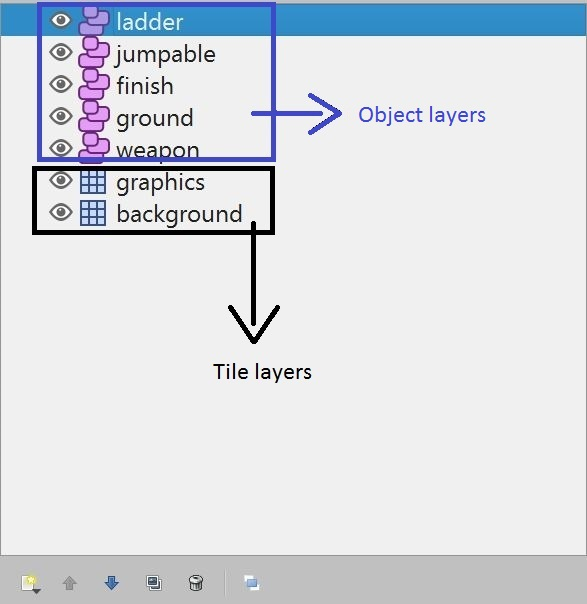
\includegraphics[width=0.5\textwidth]{Documentation/layers}
  \caption{An example of layers}
  \label{fig:ExampleOfMapLayers}
\end{figure}


After making the map in the Tiled program, we exported it in a .tmx file and used it in the project. TMX file contains all the map’s custom properties and all the layers, which has been made in the Tiled program. The following code is an example on how the .tmx file works with our project:

\begin{minted}[linenos,breaklines]{java}
// Load the first map from Tiles
mapLoader = new TmxMapLoader();

switch (gameProgress.getCurrentLevel()) {
  case 1:
    map = mapLoader.load("maps/level_1/level_1.tmx");
    break;
  case 2:
    map = mapLoader.load("maps/level_2/level_2.tmx");
    break;
  case 3:
    map = mapLoader.load("maps/boss/boss_level.tmx");
    break;
  default:
    game.exitApplication("Couldn't find level, exiting application");
    break;
}


\end{minted}


 %------------------------------------------------

\subsection{Twitch} \label{Twitch}

%----------------------------------------------------------------------------------------
%	DISCUSSION
%----------------------------------------------------------------------------------------

\newpage
\section{Discussion}

Discussion.

%----------------------------------------------------------------------------------------
%	CONCLUSION
%----------------------------------------------------------------------------------------

\newpage
\section{Conclusion}

Project Conclusion.

%----------------------------------------------------------------------------------------
%	BIBLIOGRAPHY
%----------------------------------------------------------------------------------------

\newpage
\printbibliography[heading=bibintoc,title={References}]

%----------------------------------------------------------------------------------------
%	APPENDIX
%----------------------------------------------------------------------------------------

\newpage
\appendix

\section{Appendix}

\subsection{Class diagram} \label{AppendixClassDiagramFull}

The following figure is the full class diagram of the entire project. A high resolution version can be found here: \texttt{https://i.imgur.com/6zzDp6a.png}

\begin{figure}[ht]
  \centering
  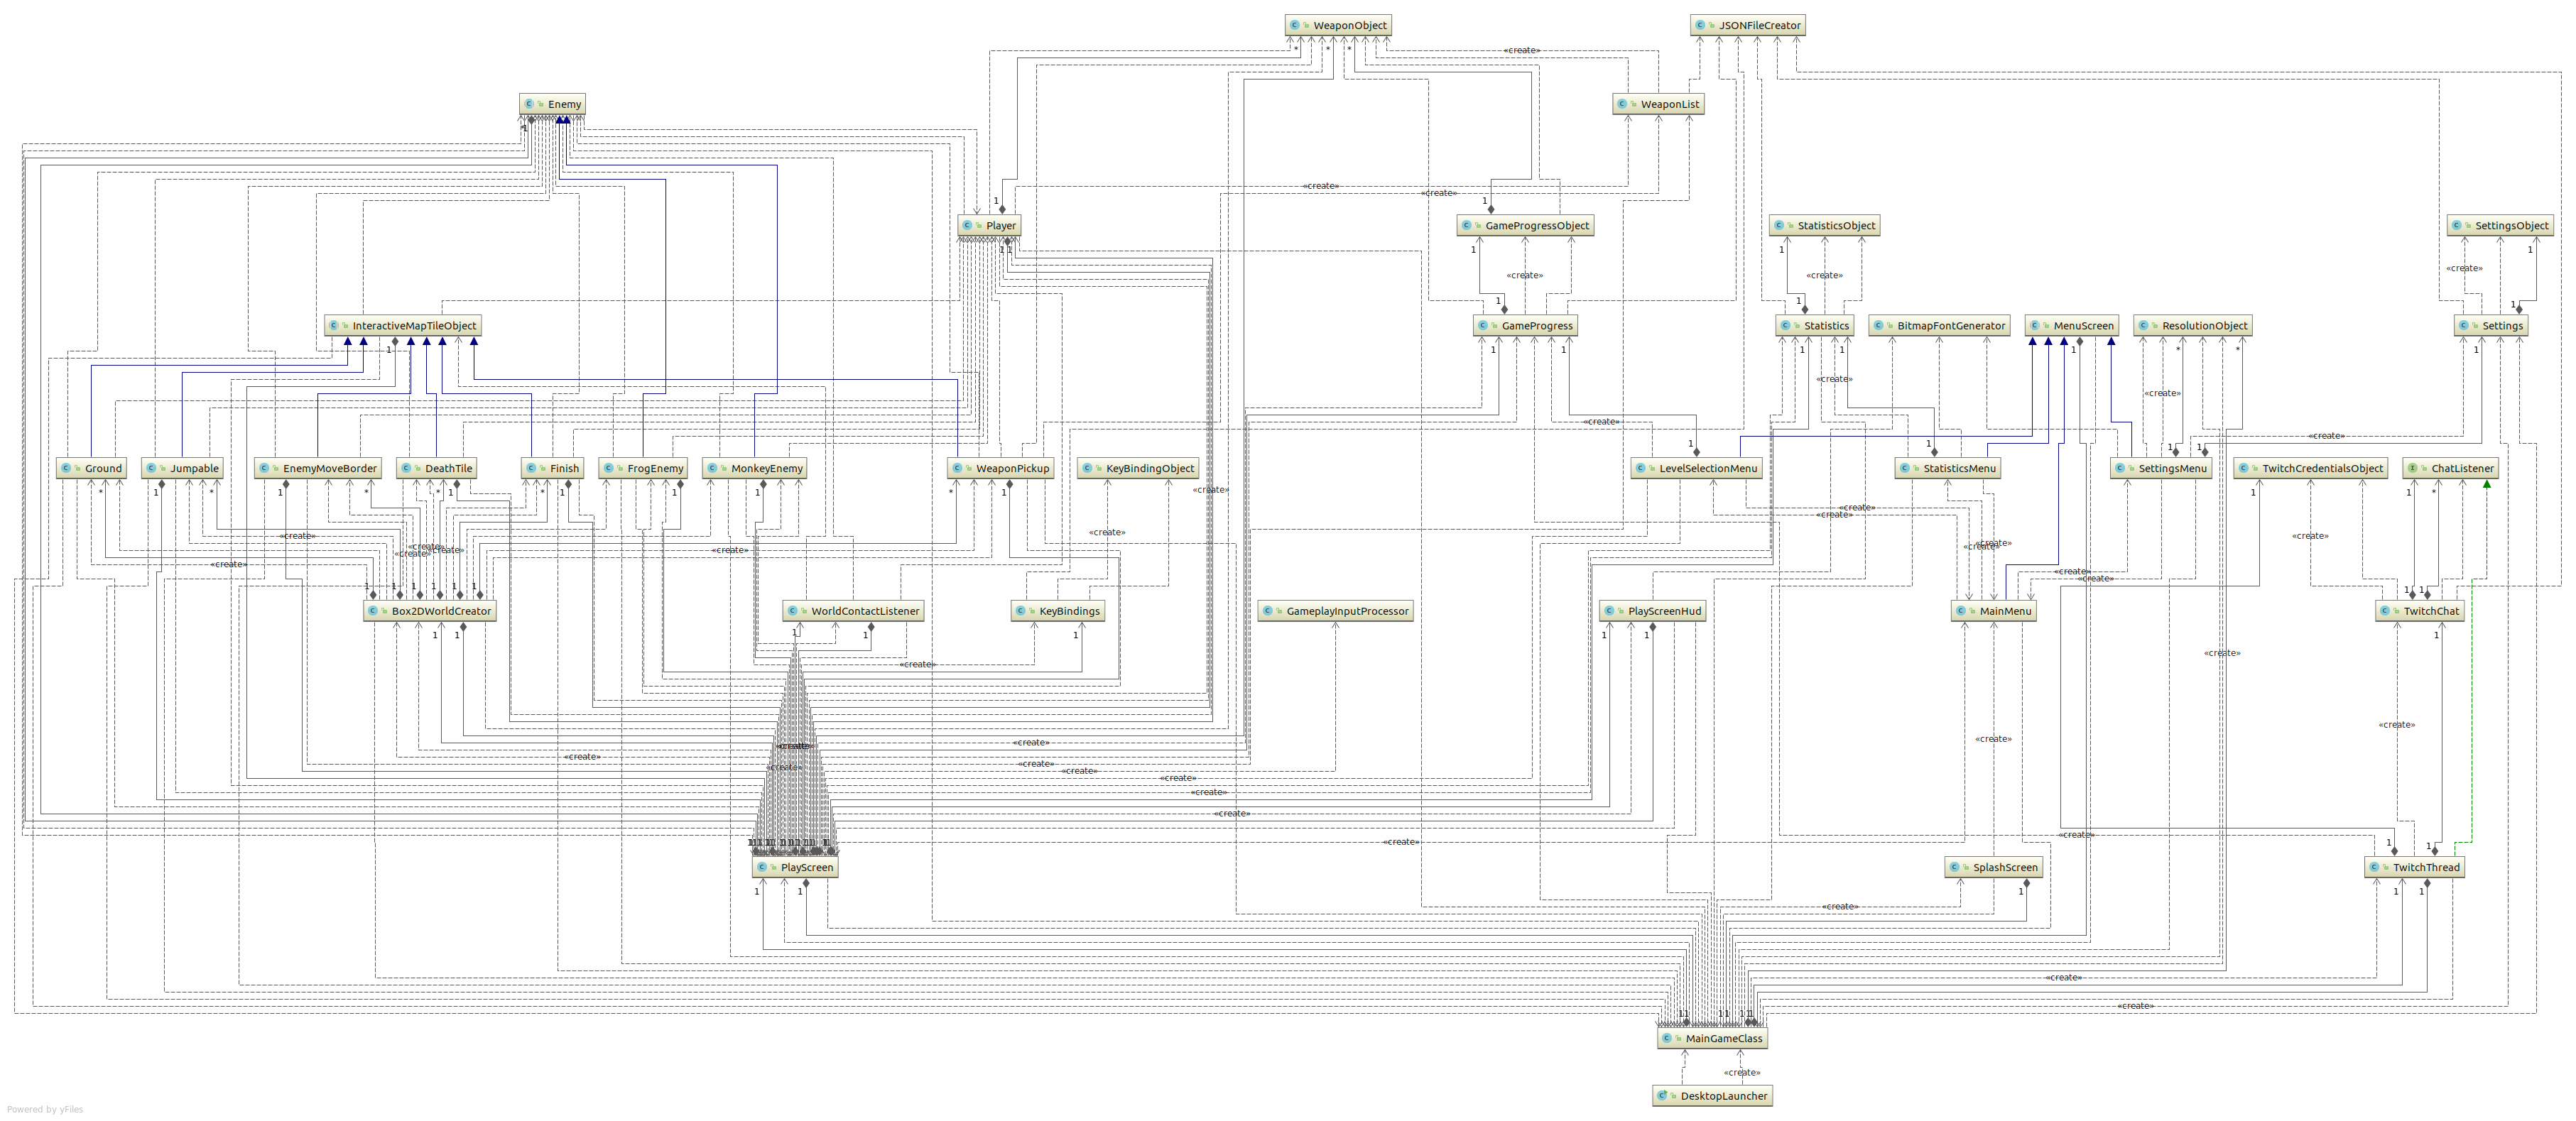
\includegraphics[width=1\textwidth]{Documentation/class_diagram}
  \caption{Full class diagram}
  \label{fig:ClassDiagramFull}
\end{figure}

%------------------------------------------------

\section{Source Code} \label{SourceCode}

The following appendix contains direct links to each Java class file and possibly other relevant files on the GitHub repository since the raw code is too long to put here.

% REMOVE IF SOMETHING ABOVE CHANGES
\newpage
% REMOVE IF SOMETHING ABOVE CHANGES

\renewcommand{\labelitemi}{\faFolderOpen}
\renewcommand{\labelitemii}{\faFile}
\renewcommand{\labelitemiii}{\faFile}
\begin{itemize}
    \item \textbf{/}
    \begin{itemize}
        \item MainGameClass: \url{https://goo.gl/sWmPjR}
    \end{itemize}
    
    \item \textbf{GameProgress}
    \begin{itemize}
        \item GameProgress: \url{https://goo.gl/2RTmRm} 
        \item GameProgressObject: \url{https://goo.gl/t1Bx4X}
    \end{itemize}
    
    \item \textbf{Input}
    \begin{itemize}
        \item GameplayInputProcessor: \url{https://goo.gl/eMSxpK}
    \end{itemize}
    
    \item \textbf{Items}
    \begin{itemize}
        \item WeaponList: \url{https://goo.gl/PysN6e}
        \item WeaponObject: \url{https://goo.gl/rUjBA5}
    \end{itemize}
    
    \item \textbf{KeyBindings}
    \begin{itemize}
        \item KeyBindingsObject: \url{https://goo.gl/FBeWNx}
        \item KeyBindings: \url{https://goo.gl/Z7PviH}
    \end{itemize}
    
    \item \textbf{Objects}
    \begin{itemize}
        \item[\faFolderOpen] \textbf{EnemyObjects}
        \begin{itemize}
            \item FrogEnemy: \url{https://goo.gl/4DGm2R}
            \item MonkeyEnemy: \url{https://goo.gl/gnWMLx}
        \end{itemize}
        
        \item[\faFolderOpen] \textbf{MapObjects}
        \begin{itemize}
            \item DeathTile: \url{https://goo.gl/6fUSQr}
            \item EnemyMoveBorder: \url{https://goo.gl/p9PvBK}
            \item Finish: \url{https://goo.gl/JEH73q}
            \item Ground: \url{https://goo.gl/uSvrrh}
            \item Jumpable: \url{https://goo.gl/fU629m}
            \item WeaponPickup: \url{https://goo.gl/KwR2Xf}
        \end{itemize}
        
        \item Enemy: \url{https://goo.gl/8zYXwP}
        \item InteractiveMapTileObject: \url{https://goo.gl/tgstsE}
        \item Player: \url{https://goo.gl/BPW542}
    \end{itemize}
    
    \item \textbf{Scenes}
    \begin{itemize}
        \item PlayScreenHud: \url{https://goo.gl/EWCC1h}
    \end{itemize}
    
    \item \textbf{Screens}
    \begin{itemize}
        \item PlayScreen: \url{https://goo.gl/qFch7g}
        \item SplashScreen: \url{https://goo.gl/LQRfX9}
    \end{itemize}
    
    \item \textbf{Statistics}
    \begin{itemize}
        \item Statistics: \url{https://goo.gl/poKVXL}
        \item StatisticsObject: \url{https://goo.gl/ZBt35J}
    \end{itemize}
    
    \item \textbf{Tools}
    \begin{itemize}
        \item BitmapFontGenerator: \url{https://goo.gl/9PTfjq}
        \item Box2DWorldCreator: \url{https://goo.gl/kZXThj}
        \item WorldContactListener: \url{https://goo.gl/xB8hMM}
    \end{itemize}
    
    \item \textbf{Twitch}
    \begin{itemize}
        \item ChatListener: \url{https://goo.gl/pPn6vq}
        \item TwitchChat: \url{https://goo.gl/d9fve2}
        \item TwitchCredentialsObject: \url{https://goo.gl/wFJnxR}
        \item TwitchThread: \url{https://goo.gl/PCXpqz}
    \end{itemize}
\end{itemize}

%------------------------------------------------

\end{document}